% arara: pdflatex: { synctex: yes }
% arara: makeindex: { style: ctuthesis }
% arara: bibtex

% The class takes all the key=value arguments that \ctusetup does,
% and a couple more: draft and oneside
\documentclass[twoside]{ctuthesis}

\ctusetup{
	% preprint = \today,
	mainlanguage = english,
	otherlanguages = {czech},
	title-czech = {Gamifikace ve výuce anglických slovíček},
	title-english = {Gamification for English Vocabulary Learning},
	subtitle-czech = {},
	subtitle-english = {},
	doctype = B,
	faculty = F3,
	department-czech = {Katedra počítačové grafiky a interakce},
	department-english = {Department of Computer Graphics and Interaction},
	author = {Petr Nejedlý},
	supervisor = {Ing. Ivo Malý, Ph.D.},
	% supervisor-address = {KN:E-425, \\ Karlovo náměstí 13, \\ Praha 2},
	fieldofstudy-english = {Software Engineering and Technology},
	subfieldofstudy-english = {Business informatics},
	fieldofstudy-czech = {Softwarové inženýrství a technologie},
	subfieldofstudy-czech = {Business informatics},
	keywords-czech = {gamifikace, anglická slovíčka, mobilní aplikace, Flutter},
	keywords-english = {gamification, English vocabulary, mobile app, Flutter},
	day = 5,
	month = 1,
	year = 2025
%	specification-file = {ctutest-zadani.pdf},
%	front-specification = true,
%	front-list-of-figures = false,
%	front-list-of-tables = false,
%	monochrome = true,
%	layout-short = true,
}

\ctuprocess

\setlength{\parskip}{1em}

\addto\ctucaptionsczech{%
	\def\supervisorname{Vedoucí}%
	\def\subfieldofstudyname{Studijní program}%
}

\ctutemplateset{maketitle twocolumn default}{
	\begin{twocolumnfrontmatterpage}
		\ctutemplate{twocolumn.thanks}
		\ctutemplate{twocolumn.declaration}
		\ctutemplate{twocolumn.abstract.in.titlelanguage}
		\ctutemplate{twocolumn.abstract.in.secondlanguage}
		\ctutemplate{twocolumn.tableofcontents}
		\ctutemplate{twocolumn.listoffigures}
	\end{twocolumnfrontmatterpage}
}

% ----- Abstract -----
\begin{abstract-czech}
TODO: tady bude abstrakt v češtině
\end{abstract-czech}

\begin{abstract-english}
TODO: here will be an abstract in English
\end{abstract-english}

% ----- Acknowledgements -----
\begin{thanks}
TODO: Acknowledgements...
\end{thanks}

% ----- Declaration -----
\begin{declaration}
TODO: Declaration...

In Prague,~\monthinlanguage{title} \ctufield{day},~\ctufield{year}
\end{declaration}

% --------------------------------------------

\begin{document}

\maketitle

% ----- THESIS TEXT (indiviual chapters) -----
\chapter{Introduction}

In today's fast-paced digital world, language learning applications have become an essential tool for individuals seeking to enhance their vocabulary and language skills. However, maintaining user engagement and motivation over time remains a significant challenge. This project addresses this issue by exploring the integration of gamification elements into the English Mind application, aiming to transform the learning experience into a more engaging and rewarding journey.

The English Mind application is built on a well-designed learning approach that effectively supports language acquisition. However, when compared to leading competitors, it falls short in terms of gamification elements. This lack of engaging features may negatively impact user motivation and retention, as users are increasingly drawn to applications that offer interactive and rewarding experiences. 

This project aims to address this gap by integrating gamification strategies that can enhance user engagement and motivation, thereby positioning English Mind more competitively in the market.

\newpage

\section{Success Criteria}

The evaluation of this work's success is structured around three principal dimensions: competitive positioning, user feedback, and implementation success. These dimensions serve as the foundation for assessing the achievement of the thesis objectives.

\begin{enumerate}
    \item \textbf{Enhancement of Competitive Positioning}
    \begin{enumerate}
        \item Analyze the English Mind vocabulary learning approach to understand the key principles of the application.
        \item Conduct analysis of gamification features used by English Mind and leading competitors.
        \item Identify opportunities for enhancing the gamification of English Mind.
    \end{enumerate}

    \item \textbf{Positive User Feedback on Gamification Features}
    \begin{enumerate}
        \item Design gamification features and elements that are on par with or surpass those of leading competitors.
        \item Conduct user testing of the new gamification features, aiming for positive feedback.
    \end{enumerate}

    \item \textbf{Successful Implementation of Gamification Features}
    \begin{enumerate}
        \item Implement the newly designed gamification features into the application.
        \item Conduct testing with end users to ensure functionality and user satisfaction.
    \end{enumerate}
\end{enumerate}

\chapter{Mobile Application English Mind}
\label{chap:mobile-application-english-mind}

English Mind is a mobile application available on Android \cite{cite:english_mind_play_store} and iOS \cite{cite:english_mind_app_store} platforms that focuses on learning English vocabulary. To achieve high efficiency in learning new English vocabulary, the application combines three main teaching methods on which it is based \cite{cite:english_mind_website}:

\begin{itemize}
    \item Frequency list of English vocabulary
    \item Active recall utilizing flashcards
    \item Spaced repetition system
\end{itemize}

These methods create a structured and efficient approach to mastering vocabulary with minimal effort, setting the app apart from its competitors in the field of vocabulary learning apps.

\section{Frequency List}

A frequency list ranks words according to their occurrence in common texts and speech. This approach is particularly valuable in vocabulary teaching for foreign language learners, as learning high-frequency words first enables students to comprehend more of their target language earlier in their studies.

Research by Nation \cite{cite:nation2006_how_large_vocabulary_is_needed} demonstrates the effectiveness of this approach. Mastering the 1,000 most frequent word families enables understanding of 78-81\% of written text, while 8,000-9,000 word families are required for 98\% comprehension. This data underscores the importance of prioritizing high-frequency vocabulary in language acquisition.\newpage

The frequency list implementation in English Mind allows users to browse words and assign them one of three states: UNSEEN (default), KNOWN, and LEARNING. Users can modify these states as shown in Figure \ref{fig:em-frequency-list}. Words marked as "LEARNING" are practiced using flashcards and scheduled for review through spaced repetition.

\begin{figure}[!h]
    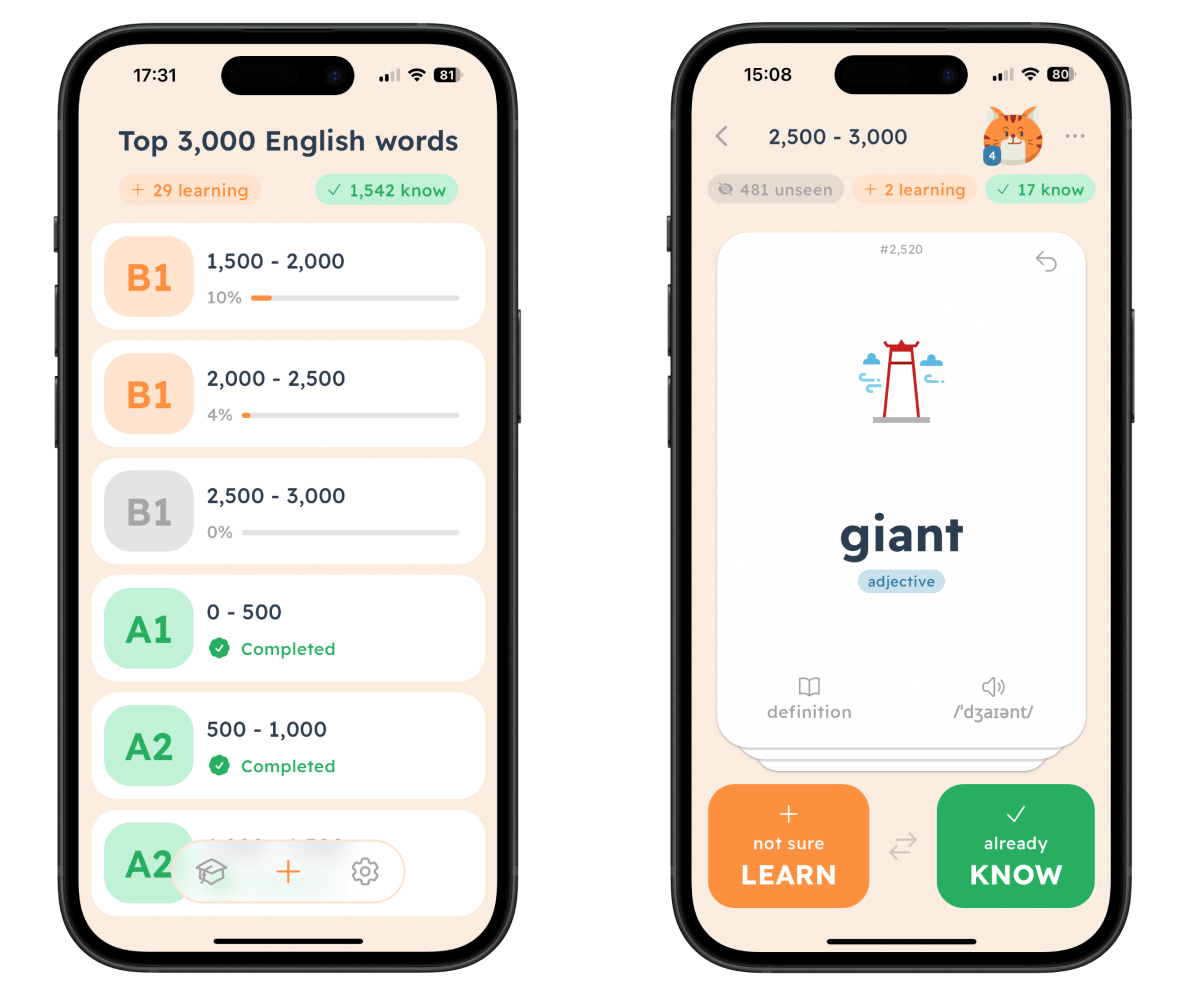
\includegraphics[width=0.8\textwidth]{src/figures/em-frequency-list.png}
    \caption{English Mind - Frequency List}
    \label{fig:em-frequency-list}
\end{figure}

\section{Active Recall and Flashcards}
\label{sec:em-active-recall}

Active recall is a learning method where students attempt to retrieve information without reference to the source material, contrasting with passive review where information is simply reread. Research from Washington University \cite{cite:rhkj2006_longterm_retention} demonstrates active recall's superiority for long-term retention: in a study of 120 students, active recall consistently outperformed passive review across various time intervals (5 minutes, 2 days, and 1 week), as shown in Figure \ref{fig:active-recall-passive-review-results}.

\begin{figure}[!h]
    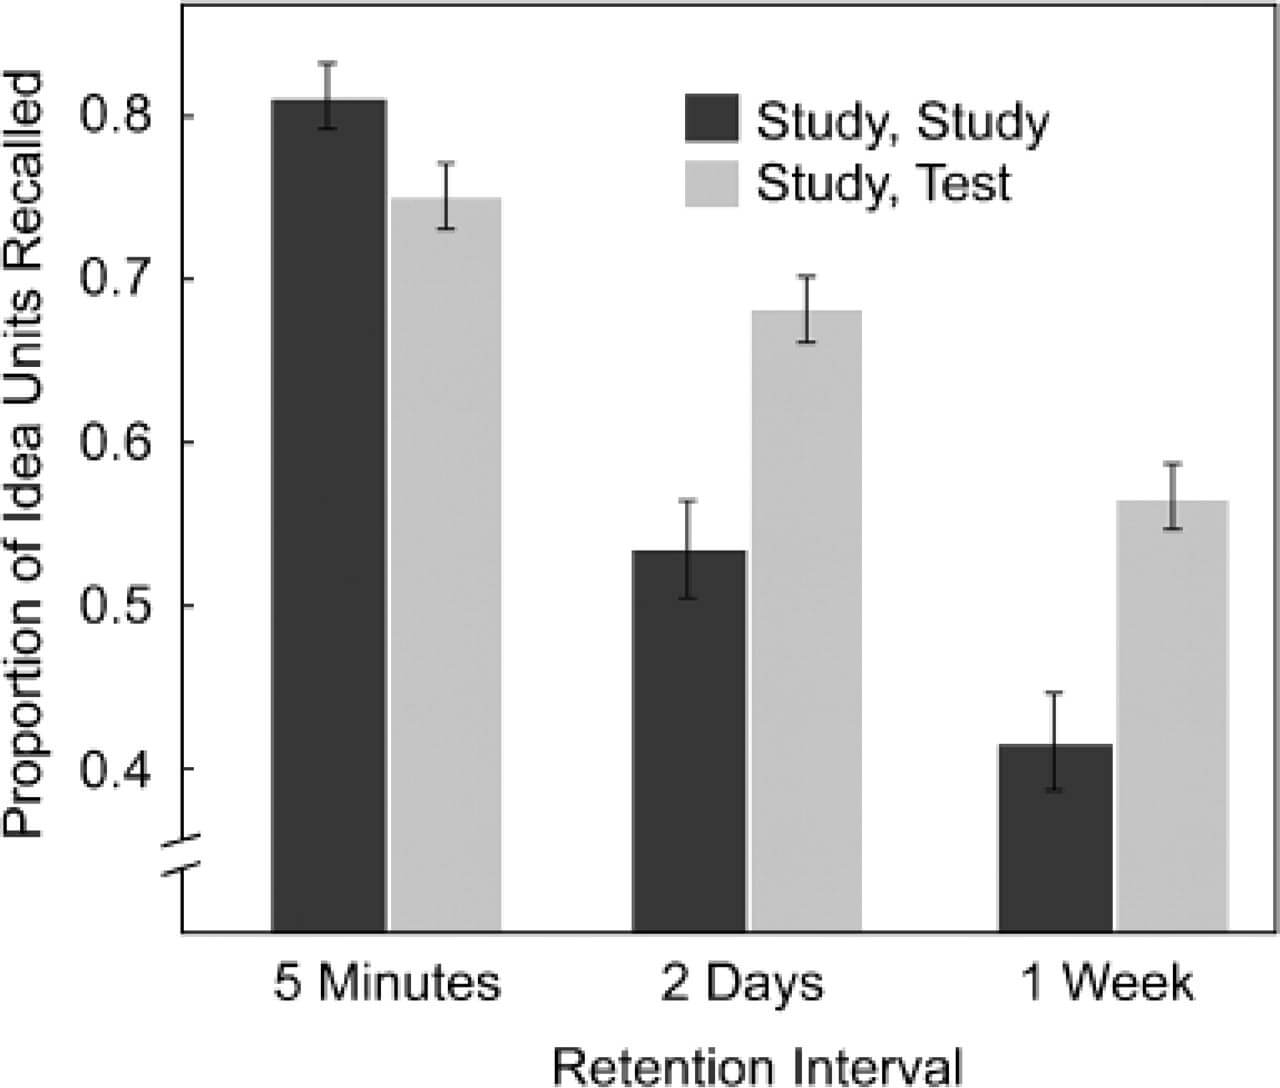
\includegraphics[width=0.7\textwidth]{src/figures/active-recall-passive-review-results.jpeg}
    \caption{Comparison of retention rates between active recall and passive review methods across different time intervals \cite{cite:rhkj2006_longterm_retention}}
    \label{fig:active-recall-passive-review-results}
\end{figure}

Flashcards represent a practical implementation of active recall, where information is split between two sides of a card, forcing active retrieval before verification.

English Mind implements flashcard-based active recall by presenting vocabulary words on the front and comprehensive word information (definition, usage examples, pronunciation, and native language translation) on the reverse, as shown in Figure \ref{fig:em-flashcards}. Users must attempt to recall the word's meaning before revealing the reverse side.

\begin{figure}[!h]
    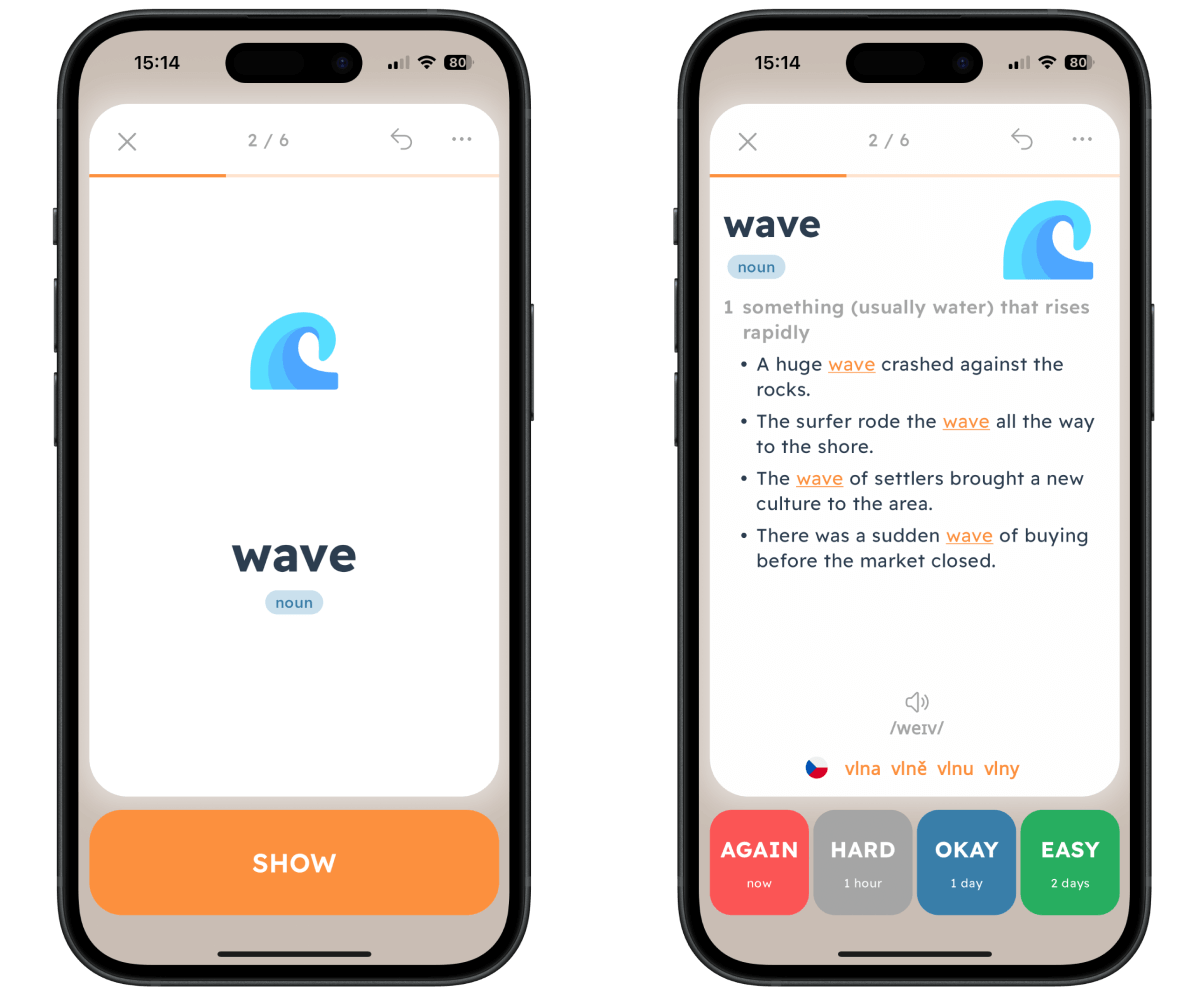
\includegraphics[width=0.9\textwidth]{src/figures/em-flashcards.png}
    \caption{English Mind - Active Recall Utilizing Flashcards}
    \label{fig:em-flashcards}
\end{figure}

\section{Spaced Repetition System (SRS)}

Spaced Repetition System (SRS) optimizes learning by adjusting intervals between review sessions based on recall performance. This method builds on Ebbinghaus's forgetting curve theory \cite{cite:ebbinghaus2013_memory_contribution_to_experimantal_psychology}, which demonstrates that information retention improves when review occurs just before predicted forgetting. Research shows that SRS increases learning efficiency by optimizing review timing and reducing unnecessary repetition \cite{cite:kang2016_spaced_repetiton_promotes_efficient_learning}.

The application implements SRS through a four-button feedback system (AGAIN, HARD, OKAY, EASY) that appears after each flashcard review, as shown in Figure \ref{fig:em-srs-flashcard}. Each button adjusts the next review interval: AGAIN and HARD decrease it, while OKAY and EASY increase it. Words consistently recalled over several months automatically transition from "LEARNING" to "KNOWN" status.

\begin{figure}[!h]
    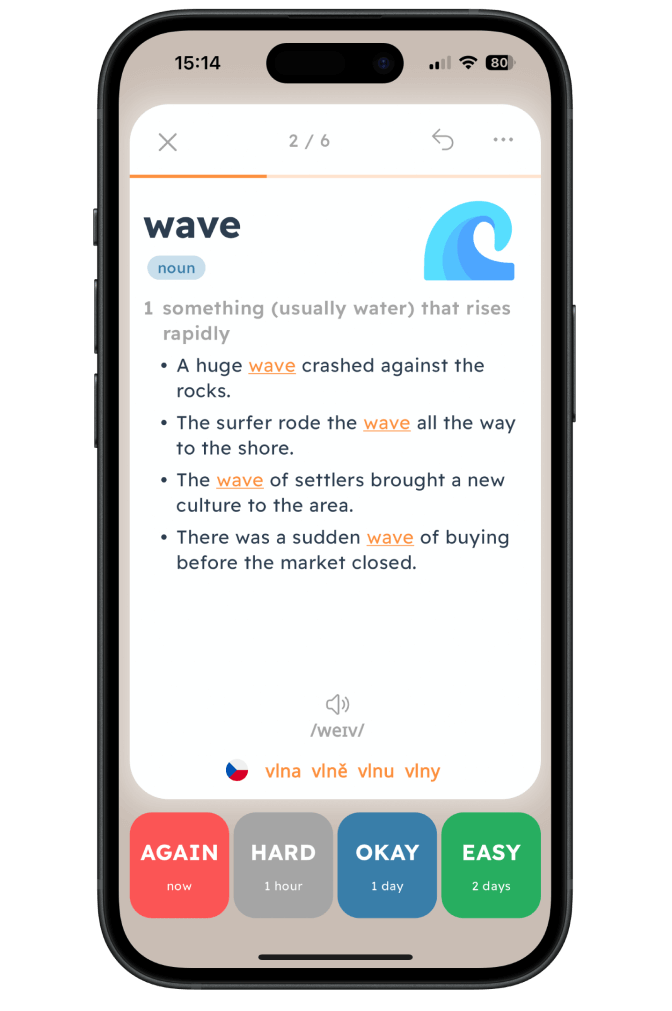
\includegraphics[width=0.6\textwidth]{src/figures/em-srs-flashcard.png}
    \caption{English Mind - SRS}
    \label{fig:em-srs-flashcard}
\end{figure}

\section{Application Workflow}

The application's learning process consists of two primary phases: vocabulary selection and practice. Figure \ref{fig:em-hta} illustrates the hierarchical breakdown of these tasks.

Users first browse the frequency-ordered vocabulary list, marking words as either "KNOWN" (already mastered) or "LEARNING" (to be studied). This initial classification ensures that learning efforts focus on appropriate vocabulary. Subsequently, words marked as "LEARNING" enter the practice phase, where they are studied through flashcards and systematically reviewed using spaced repetition.

\vspace{1cm}

\begin{figure}[!h]
    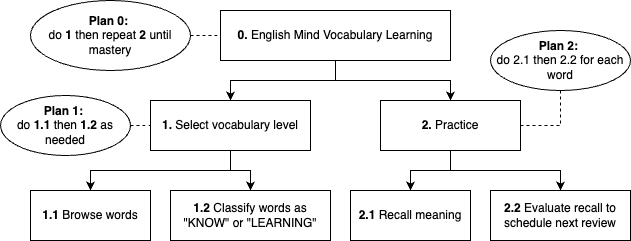
\includegraphics[width=1\textwidth]{src/figures/english_mind_workflow_THA.png}
    \caption{English Mind - Hierarchical Task Analysis of the core learning workflow}
    \label{fig:em-hta}
\end{figure}


\part{Analysis}
\chapter{Analysis of Gamification in Language Learning Applications}

Gamification is defined as "the use of game design elements in non-game contexts" \cite{cite:deterding2011_gamefulness}. In educational contexts, gamification enhances learning activities with game mechanics to boost student engagement and motivation. This strategy has become increasingly popular, especially within language learning applications.

Traditional methods of vocabulary learning, such as mechanical repetition or passive reading, can often be monotonous and lead to a decline in interest. Gamification brings these methods to life through elements such as rewards, challenges and competitions, creating an environment that encourages repeated and focused learning. This approach not only increases intrinsic learner's motivation but also helps students retain vocabulary more effectively in the long term.

Gamification includes a vast array of concepts, like streaks, badges, achievements, challenges, quests, leaderboards, rewards, statistics, progression tracking, levels and tiers, user-generated content, time-limited events, feedback loops, personalization, social elements, narrative and storytelling, virtual currencies, and so on \cite{cite:govender2021_gamification_elements_in_language_learning_apps}. Furthermore, all of them can be combined and mixed in various ways. Therefore, we will focus on a selected few that can significantly enhance the user experience in the English Mind app rather than trying to cover every single gamification concept that could benefit vocabulary learning.

\newpage

\section{Current Gamification in English Mind}

English Mind currently lacks extensive gamification features, relying instead on a few elements that can be classified as basic forms of gamification. We have identified three such elements:

\begin{itemize}
    \item \textbf{Progress Tracking of Vocabulary Acquisition} 
    \label{chap:em-progess-tracking-of-vocabulary-aquisition}
    
    Users can view essential statistics regarding their vocabulary acquisition, including the number of words they already know, the number they are currently learning, and the total remaining words to uncover. These statistics are accessible on both the vocabulary levels overview screen and on the specific vocabulary level screen.

    \begin{figure}[!h]
        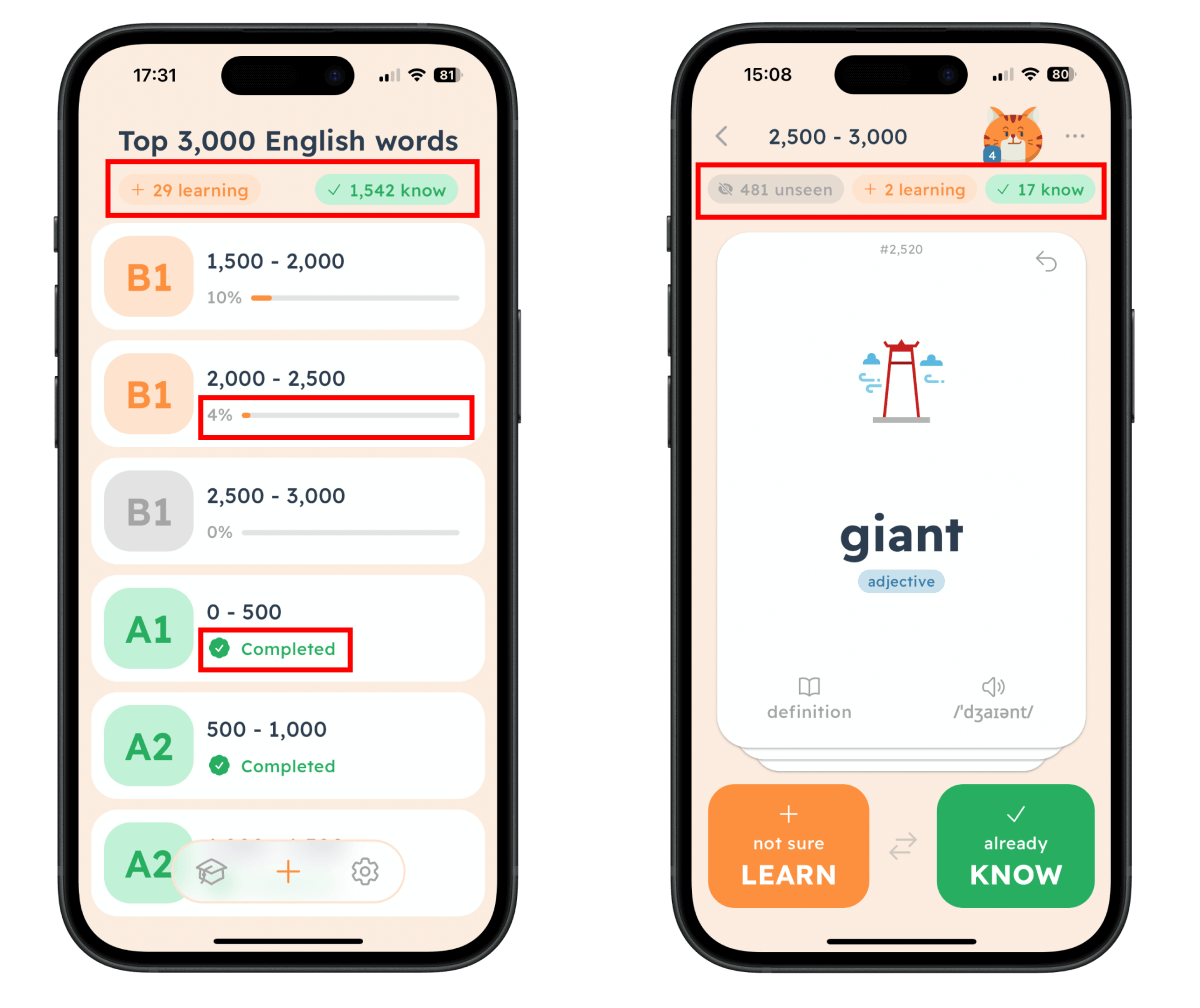
\includegraphics[width=1.1\textwidth]{src/figures/em-progress-tracking.png}
        \caption{English Mind - Progress Tracking of Vocabulary Acquisition (highlighted in red)}
        \label{fig:em-progress-tracking}
    \end{figure}

    \newpage

    \item \textbf{Daily Goal}
    \label{chap:em-daily-goal}
    
    During an onboarding process, users set a personal goal for the number of new words they wish to start learning each day. This personalized approach helps users maintain a sustainable learning pace while providing a clear daily objective. Setting achievable goals can increase motivation and create a sense of accomplishment when met.

    Additionally, a mascot appears in the top right corner on the word addition screen to count the newly added words awaiting their first practice session (see Figure \ref{fig:em-daily-goal}). This mascot serves a dual purpose, it tracks word additions and helps ensure that users do not overwhelm themselves by adding too many new words to learn at once.

    \begin{figure}[!h]
        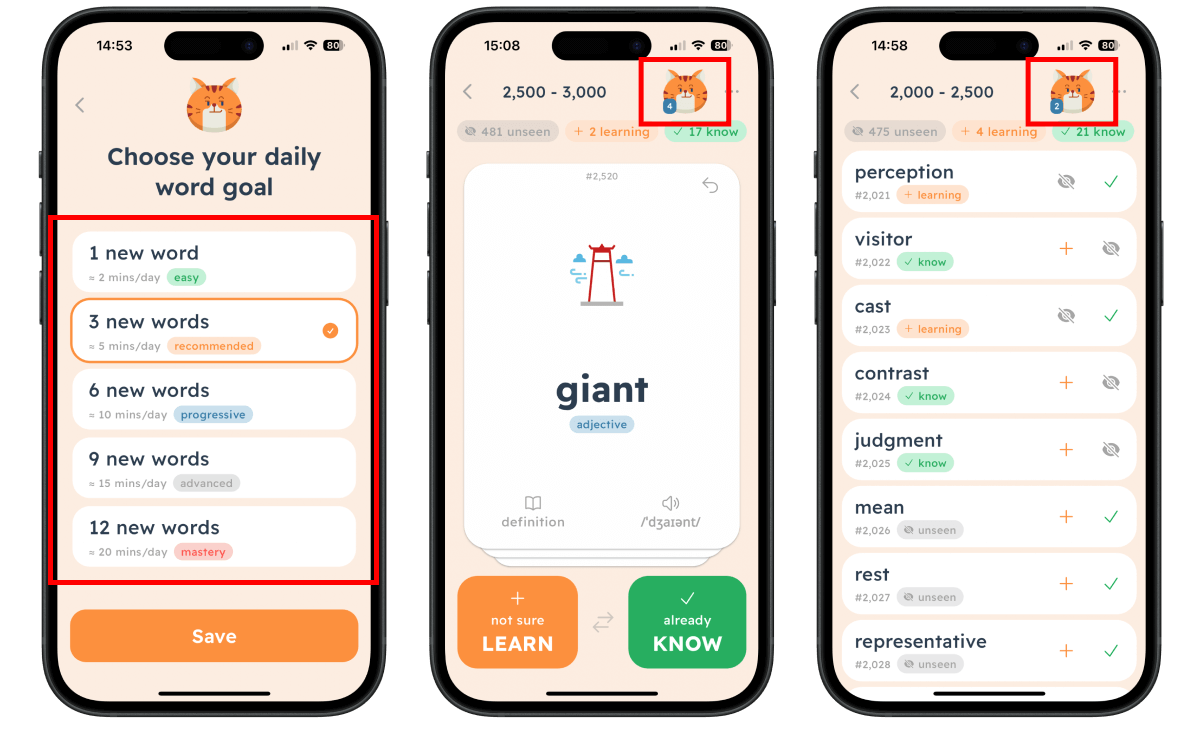
\includegraphics[width=1.05\textwidth]{src/figures/em-daily-goal.png}
        \caption{English Mind - Daily Goal and Word Addition Tracker (both highlighted in red)}
        \label{fig:em-daily-goal}
    \end{figure}


    \item \textbf{Progress Bar}
    
    While learning vocabulary through the daily queue of flashcards, users are presented with a progress bar that visually indicates their advancement, which gives them instant feedback as they progress and might motivate them to finish the current daily queue of flashcards (see Figure \ref{fig:em-flashcards-progress-bar}). Although this is a minor gamification feature, it is noteworthy given the app’s limited implementation of gamification elements.

    \newpage

    \begin{figure}[!h]
        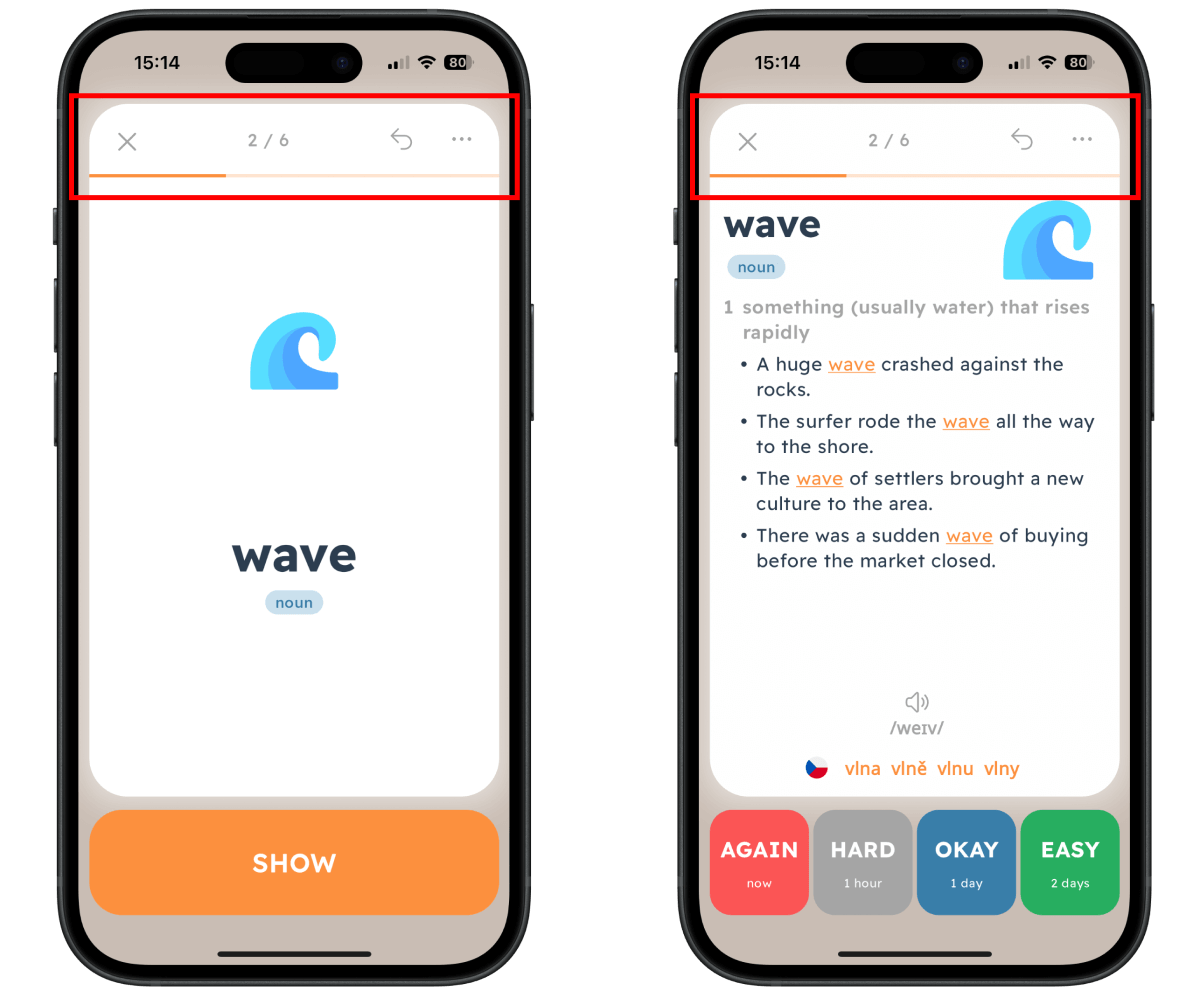
\includegraphics[width=1.05\textwidth]{src/figures/em-flashcards-progress-bar.png}
        \caption{English Mind - Progress Bar (highlighted in red)}
        \label{fig:em-flashcards-progress-bar}
    \end{figure}
    
\end{itemize}

In summary, there is potential to enhance the app by developing a more comprehensive gamification framework, which could further enrich the user experience and encourage greater motivation for improved learning outcomes.

\newpage

\section{Gamification in Similar Applications}

Before proposing new gamification features for the English Mind app, we decided to briefly analyze three mobile apps that either closely align with its learning concepts, as discussed in Chapter \ref{chap:mobile-application-english-mind}, or demonstrate innovation in the field of gamification. The selected applications are: 

\begin{itemize}
    \item \textbf{WordUp} \cite{cite:wordup}

    This app closely resembles English Mind in terms of learning concepts, as it also combines flashcards with frequency lists and a spaced repetition system.

    \item \textbf{DuoCards} \cite{cite:duocards}

    DuoCards is similar to English Mind, utilizing both flashcards and a spaced repetition system, but it lacks the incorporation of frequency lists.

    \item \textbf{Duolingo} \cite{cite:duolingo}

    While Duolingo is not based on the same learning concepts as English Mind, it was chosen for its extensive use of gamification elements and its innovations in the field. These features offer valuable inspiration for potential enhancements.
    
\end{itemize}

The following subsections will briefly explore the gamification elements used in each of these apps.

\subsection{WordUp}

WordUp application is particularly relevant as it utilizes the same learning concepts as English Mind and could inspire new gamification strategies that further support and enhance these concepts. The app has over 5 million downloads on Google Play with an average rating of 4.5 stars \cite{cite:wordup_google_play}, making it one of the most downloaded apps in English language learning field.

The app's gamification analysis identified relatively fewer gamification features despite its popularity. The vast majority of the elements identified were related in some way to practicing the flashcards queue. In the area of adding new words, a single gamification element was identified. Namely, the progress completion of a particular vocabulary range, which is very similar to the \textit{progress tracking of vocabulary acquisition} \ref{chap:em-progess-tracking-of-vocabulary-aquisition} in English Mind; therefore, it will not be listed.

Identified gamification elements are:

\newpage

\begin{itemize}
    \item \textbf{Various Types of Flashcards}

     WordUp uses four different types of flashcards that are rotated regularly to break the stereotype of flashcard practice. Each flashcard type focuses on a different aspect of learning acquisition or its combination, such as meaning, spelling, and listening. This approach effectively mitigates the monotony often associated with traditional flashcard practice, thereby increasing user engagement and interest. The four types of flashcard are (see Figure \ref{fig:wordup-flashcard-types}):
    
    \begin{itemize}
        \item \textbf{Read a word and choose the correct definition}
        
        Promotes word comprehension by having users select the most accurate definition, reinforcing meaning and usage.
        
        \item \textbf{Read a definition and choose the correct word}

        Strengthens recall by prompting users to match the definition with the correct term.
        
        \item \textbf{Read a definition and choose the correct spelling}

        This type emphasizes spelling accuracy, requiring users to focus on the correct letter sequence while associating the word with its meaning.
        
        \item \textbf{Listen to a word and choose the correct spelling}

        Enhances auditory skills and spelling, as users select the correct spelling of the spoken word.
        
    \end{itemize}

    \begin{figure}[!h]
        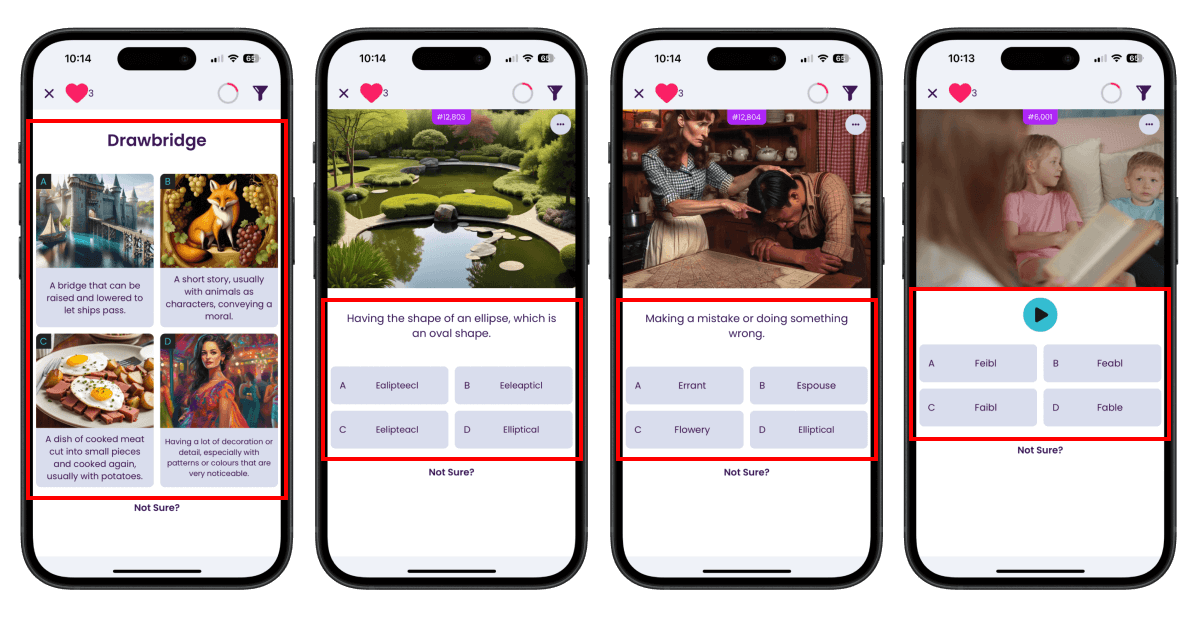
\includegraphics[width=1\textwidth]{src/figures/wordup-flashcard-types.png}
        \caption{WordUp - Types of Flashcards (highlighted in red)}
        \label{fig:wordup-flashcard-types}
    \end{figure}
    
    \item \textbf{Progress tracking for individual words}
    \label{sec:wordup-individual-word-progress-experience}
    
    WordUp uses its own unique spaced repetition system. It features a visual indicator that tracks each word's progress, showing how many times the user has correctly recalled it (see Figure \ref{fig:wordup-word-progress}). This interactive feedback motivates continued practice, rewarding users with a sense of achievement as they advance.

    \begin{figure}[!h]
        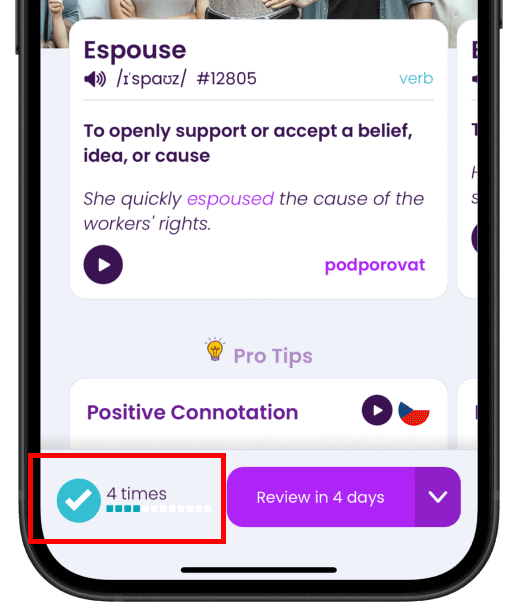
\includegraphics[width=0.35\textwidth]{src/figures/wordup-word-progress.png}
        \caption{WordUp - Indicator of Word's Progress (highlighted in red)}
        \label{fig:wordup-word-progress}
    \end{figure}

    \item \textbf{Daily Goal and Leaderboard}

    WordUp introduces a daily goal based on minutes spent practicing to motivate users to practice regularly. First, the user sets a daily commitment for how many minutes they intend to practice English vocabulary. Each day, they strive to complete a circular progress ring representing this goal, providing a clear sense of accomplishment (see Figure \ref{fig:wordup-daily-goal}).
    
    Additionally, WordUp includes a leaderboard that ranks users based on the minutes they spend practicing (see Figure \ref{fig:wordup-daily-goal}). Users can compare their achievements with friends or other learners, adding a social and competitive element that encourages continued practice. 

    \begin{figure}[!h]
        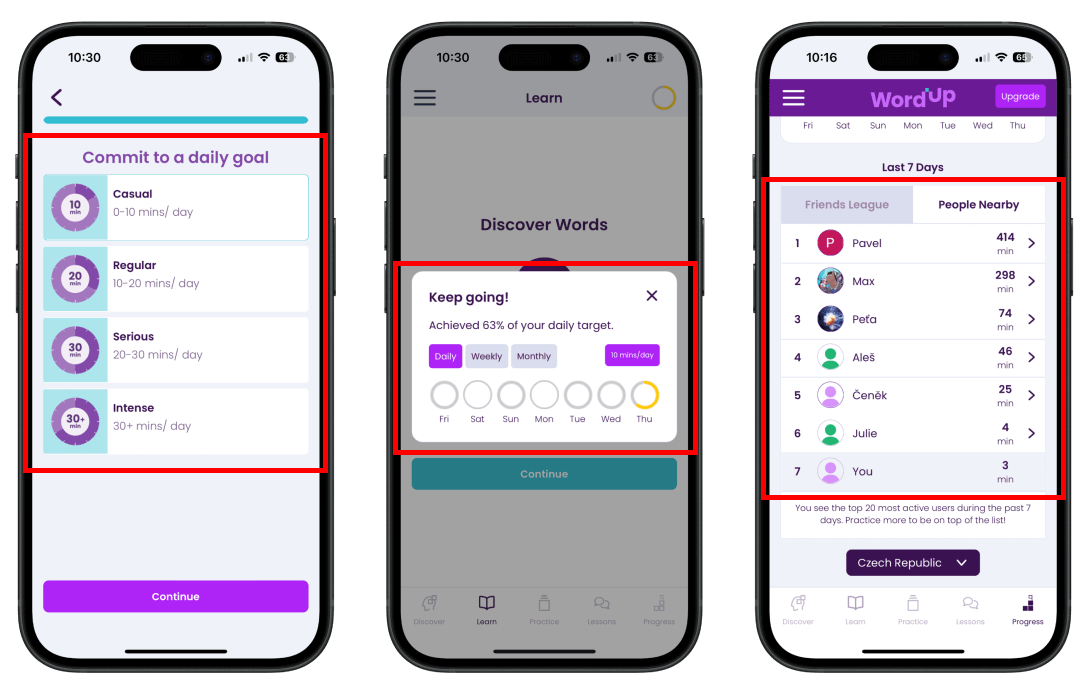
\includegraphics[width=0.99\textwidth]{src/figures/wordup-daily-goal.png}
        \caption{WordUp - Daily Goal and Leaderboard (both highlighted in red)}
        \label{fig:wordup-daily-goal}
    \end{figure}

\end{itemize}

\subsection{DuoCards}

The DuoCards application uses an SRS-based flashcard approach for vocabulary practice and has over a million downloads on Google Play with an average rating of 4.6 stars \cite{cite:duocards_google_play}. 

The analysis of gamification features reveals two key concepts: various types of flashcards and a more complex mascot upgrade system using virtual currency. The following sections provide detailed descriptions of these two concepts.

\begin{itemize}
    \item \textbf{Various Types of Flashcards}

    Duocards utilizes four different types of flashcards (see Figure \ref{fig:duocards-flashcard-types}) to keep practice exciting and address various aspects of language acquisition, such as spelling and meaning. This gamified approach maintains user interest, enhancing the learning experience. Identified flashcard variants are:

    \begin{itemize} 
         \item \textbf{English to Native Language}
         
         Displays an English word on the front, with its translation on the back. 

         \item \textbf{Native Language to English}
         
         Reverses the direction, showing the native language word on the front and prompting the English translation on the back.
         
        \item \textbf{Pronunciation Focus}
        
        Emphasizes auditory learning by presenting only the word’s pronunciation, with spelling revealed upon flipping the flashcard. 
        
        \item \textbf{Matching Exercise}
        
        Appears periodically, involving the matching of five words with their correct translations. 
    
    \end{itemize}

    \begin{figure}[!h]
        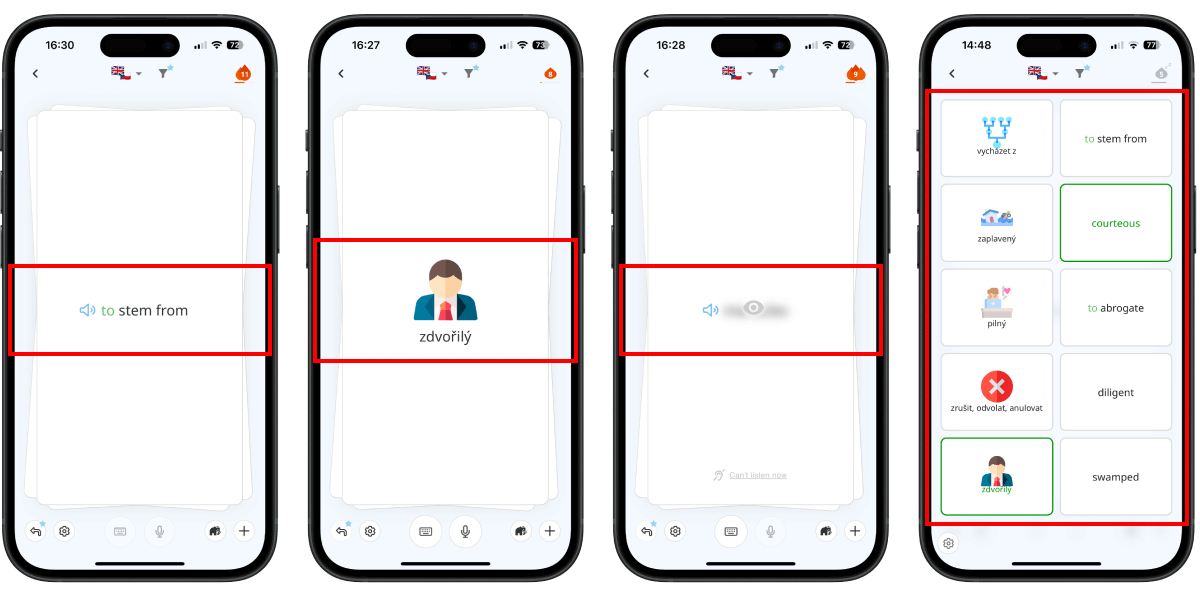
\includegraphics[width=0.98\textwidth]{src/figures/duocards-flashcard-types.png}
        \caption{DuoCards - Types of Flashcards (highlighted in red)}
        \label{fig:duocards-flashcard-types}
    \end{figure}
    
    \item \textbf{Mascot Upgrade System and Virtual Currency}

    The app’s most intriguing gamification feature is its mascot, Memo, which lives in a customizable habitat on the main screen. Users can upgrade Memo’s home by purchasing and arranging various items, creating a personalized space for them. These upgrades require a virtual currency, XP (Experience Points), which users earn by practicing and adding new vocabulary. This system rewards learning progress and adds a creative, interactive layer to vocabulary practice.

    By engaging users in developing Memo’s habitat, the app stimulates a sense of ownership and investment in the learning process. This connection can enhance motivation and commitment to vocabulary acquisition, making learning feel more like a game than a chore. 

    \begin{figure}[!h]
        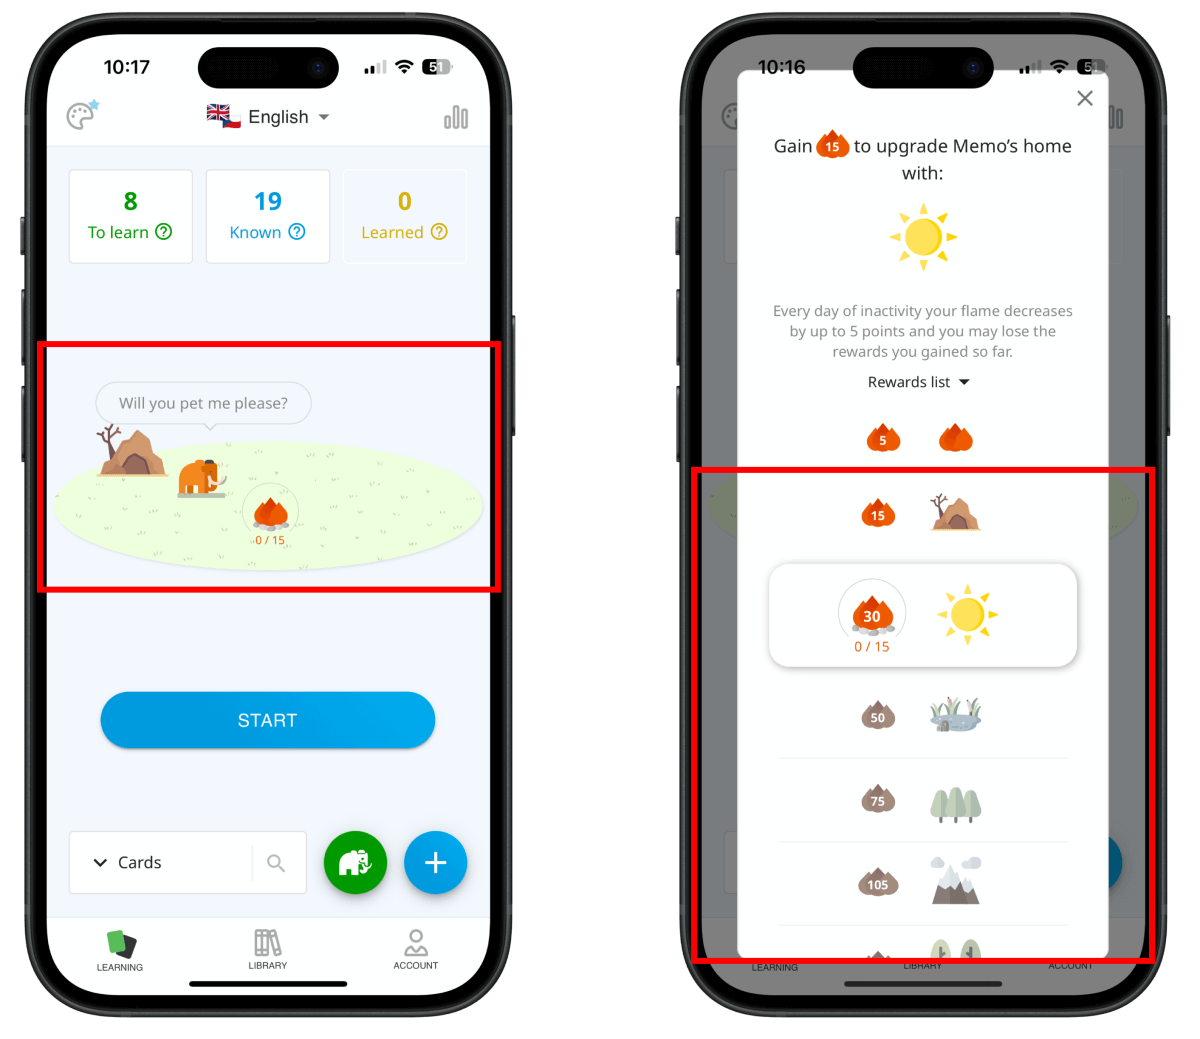
\includegraphics[width=0.7\textwidth]{src/figures/duocards-memo.png}
        \caption{DuoCards - Mascot Upgrade System (highlighted in red)}
        \label{fig:duocards-memo}
    \end{figure}

\end{itemize}

\subsection{Duolingo}

Duolingo, the world's most popular language learning application with over 100 million monthly active users \cite{cite:duolingo_2024q2}, has revolutionized digital language education through its accessible and engaging approach. The application was chosen for analysis due to its pioneering innovations in gamification. While numerous studies have examined Duolingo's gamification strategies, we will focus only on a few elements that could be effectively adapted for English Mind, particularly those that complement its learning concepts and methodologies.

Analysis revealed three concepts that English Mind could benefit from if implemented effectively. The following sections provide an introduction to these concepts.

\begin{itemize}
    \item \textbf{Various Exercises}

    Duolingo structures its content into bite-sized lessons, each consisting of a series of varied exercises similar to interactive flashcards. The variety of exercises keeps users engaged as they practice. Some of these exercises include:

    \begin{itemize}
        \item \textbf{Matching pairs}

        In this exercise, users are presented with a set of five words and their translations, which they must correctly pair together (see Figure \ref{fig:duolingo-exercise-types}). This matching activity typically appears at regular intervals throughout lessons or after the introduction of new vocabulary.
        
        \item \textbf{Speaking practice}

        Users are presented with a sentence to pronounce, and Duolingo's speech recognition system automatically evaluates their attempts (see Figure \ref{fig:duolingo-exercise-types}). This speaking practice feature is particularly noteworthy, as many applications traditionally avoid incorporating speech exercises due to the technical challenges of natural language processing. However, with recent advancements in Large Language Models (LLMs) and their increasing accessibility, the integration of speech exercises is becoming more feasible.
        
        \item \textbf{Spelling practice}

        Users are presented with an audio recording of a sentence and must transcribe it accurately, focusing on proper spelling of each word. This exercise reinforces both listening comprehension and spelling skills (see Figure \ref{fig:duolingo-exercise-types}).
    \end{itemize}

    \begin{figure}[!h]
        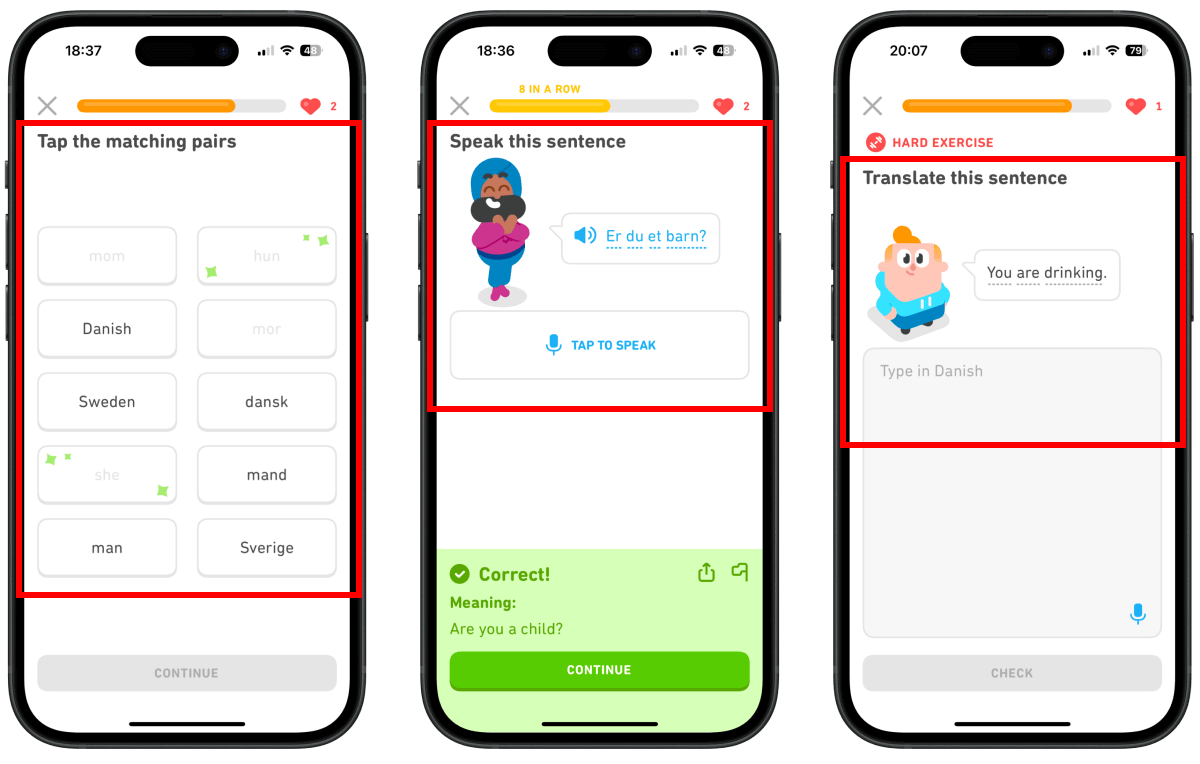
\includegraphics[width=0.98\textwidth]{src/figures/duolingo-exercise-types.png}
        \caption{Duolingo - Types of Exercises (highlighted in red)}
        \label{fig:duolingo-exercise-types}
    \end{figure}

    \item \textbf{Short Review After Finishing a Lesson}
    \label{sec:duolingo-lesson-review}

    After completing each lesson, Duolingo presents users with an engaging summary screen accompanied by a celebratory animation (see Figure \ref{fig:duolingo-lesson-review}). The summary includes key metrics such as:

    \begin{itemize}
        \item Experience points (XP) earned
        \item Accuracy rate for the completed exercises
        \item Time spent practicing
        \item Maintenance of learning streaks
    \end{itemize}

    This immediate feedback loop is crucial for user motivation, as it provides a sense of achievement and progress tracking. The inclusion of XP points and streaks transforms the learning process into a game-like experience, encouraging users to maintain consistent practice habits. The celebratory animations and positive reinforcement help create a rewarding atmosphere, making the learning process more enjoyable.

    \begin{figure}[!h]
        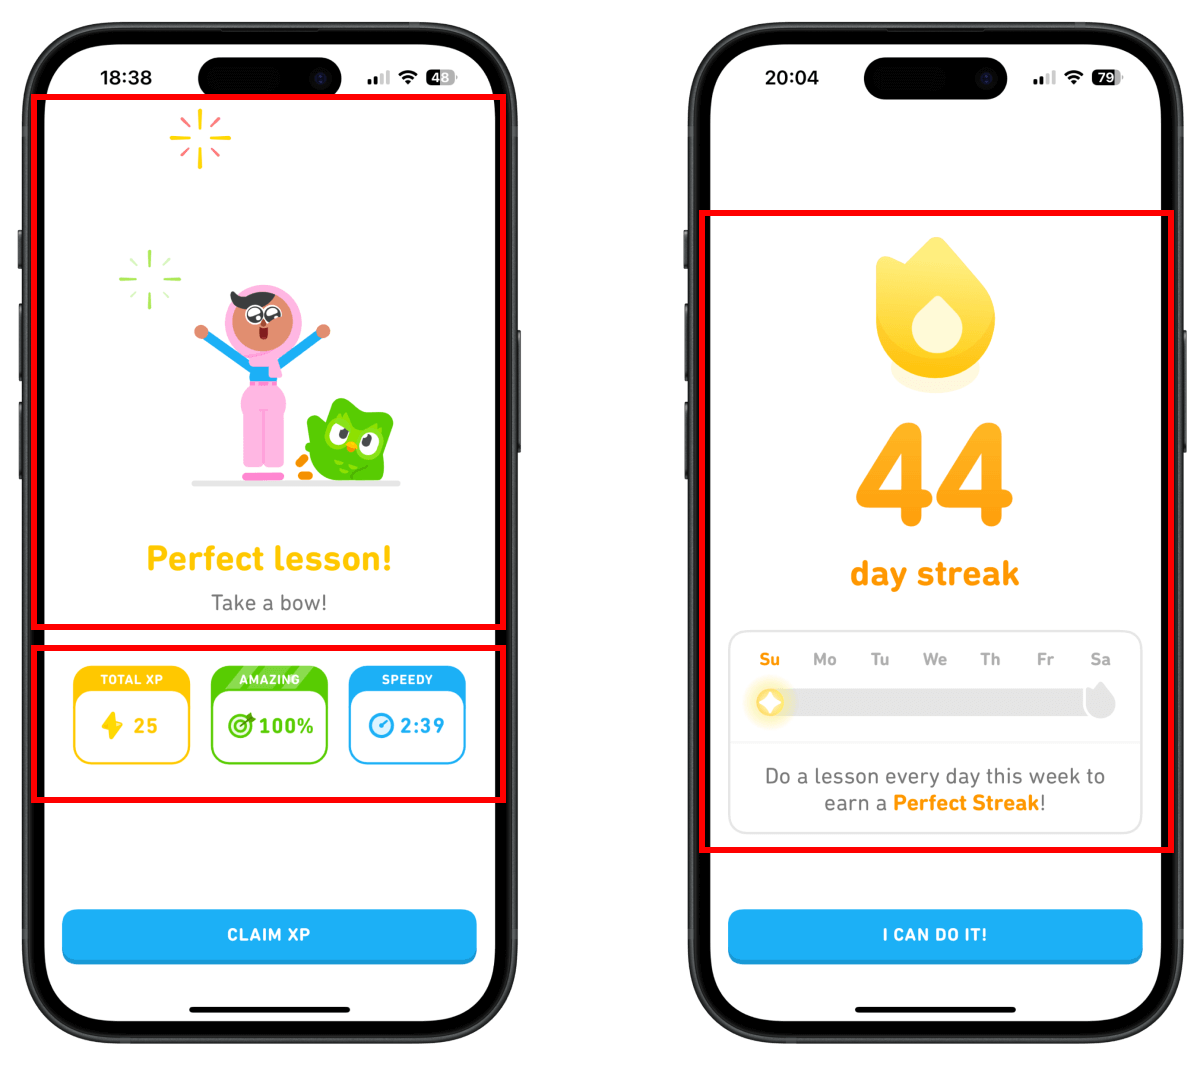
\includegraphics[width=0.85\textwidth]{src/figures/duolingo-lesson-review.png}
        \caption{Duolingo - Review After Finishing a Lesson (highlighted in red)}
        \label{fig:duolingo-lesson-review}
    \end{figure}

    \newpage

    \item \textbf{Daily Streak}
    \label{sec:duolingo-streak-system}

    One of Duolingo's most powerful gamification features is the daily streak system, which tracks consecutive days of learning activity (see Figure \ref{fig:duolingo-daily-streak}). Users maintain their streak by completing at least one lesson each day, creating a powerful psychological incentive for consistent practice. To make this system more flexible and user-friendly, Duolingo introduced "Streak Freezes" - items that users can acquire to preserve their streak during a day of inactivity.

    \begin{figure}[!h]
        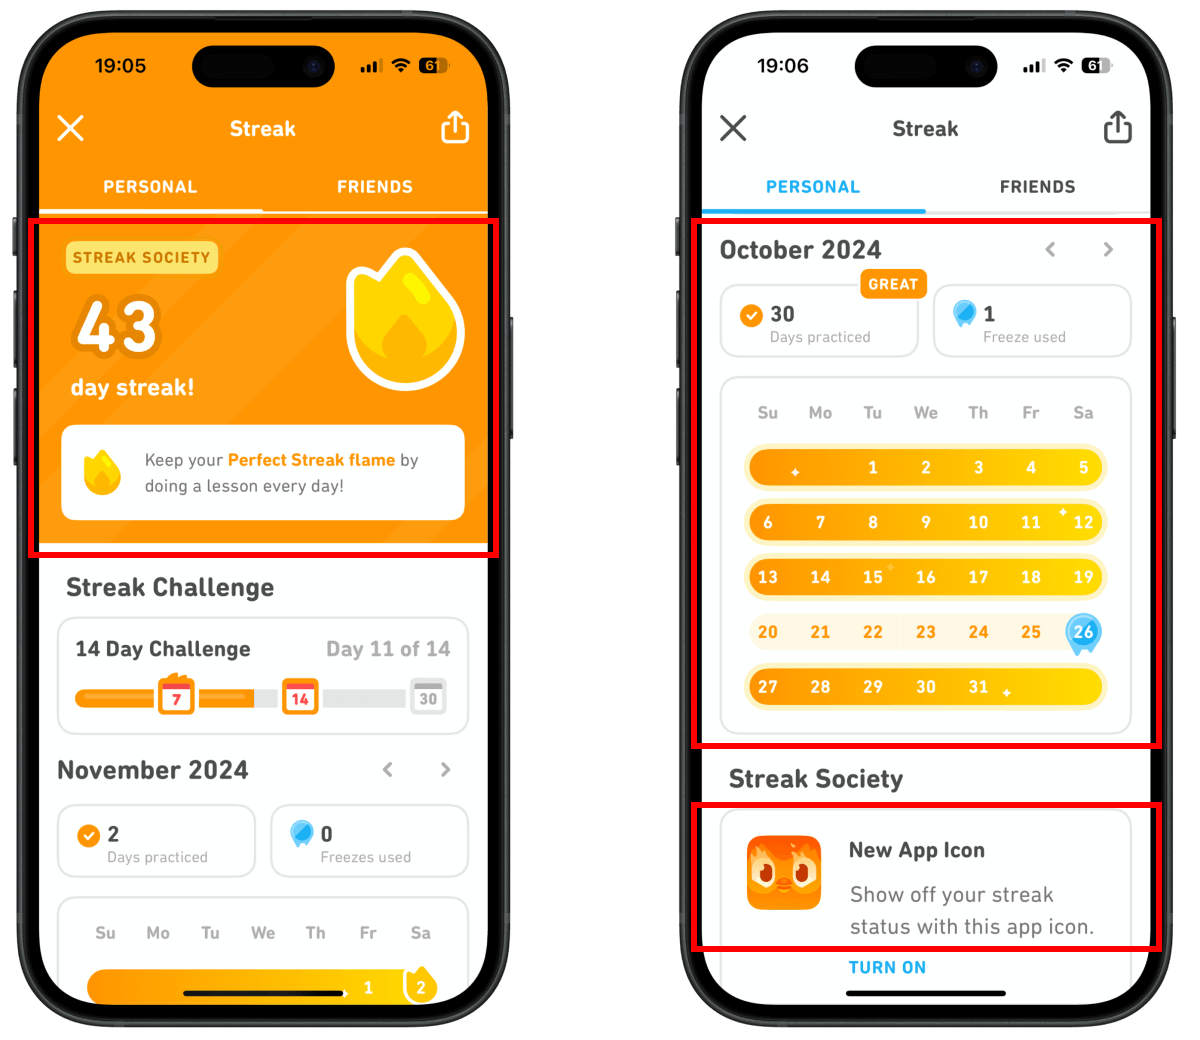
\includegraphics[width=0.72\textwidth]{src/figures/duolingo-streak.png}
        \caption{Duolingo - Daily Streak (highlighted in red)}
        \label{fig:duolingo-daily-streak}
    \end{figure}

    The streak system is supported by a sophisticated notification framework that employs various psychological triggers to maintain user engagement. These include:

    \begin{itemize}
        \item Reminder notifications at user-specified times
        \item Warnings when streaks are at risk of breaking
        \item Motivational messages to encourage streak continuation
        \item Interactive home screen widgets displaying streak counts
        \item Celebrations of streak milestones
        \item Collectible app icons that unlock at different streak milestones
    \end{itemize}

    These features work together to create multiple touchpoints throughout the user's day, combining immediate rewards with long-term achievement tracking. The effectiveness of this approach is evident in the data. Over 20\% of Duolingo's daily active users maintain streaks longer than one year \cite{cite:duolingo_2024q2}. The streak system exemplifies how gamification can transform a learning obligation into an engaging daily ritual, effectively addressing one of language learning's most significant challenges: maintaining a consistent practice.
    
\end{itemize}

\section{Comparison and Findings}

The analysis of gamification features across English Mind and similar applications reveals several interesting patterns and opportunities for enhancement. Table \ref{tab:gamification-comparison} provides a comprehensive overview of the features implemented across all analyzed applications, highlighting both commonalities and unique approaches.

\begin{table}[h]
    \caption{Comparison of Gamification Features Across Applications}
    \label{tab:gamification-comparison}
    
    % Spacing between rows and columns
    \renewcommand{\arraystretch}{1.2}
    \setlength{\tabcolsep}{2pt}
    
    \begin{tabular}{l>{\centering}p{2cm}>{\centering}p{2cm}>{\centering}p{2cm}>{\centering\arraybackslash}p{2cm}}
        \toprule
        \textbf{Feature} & \textbf{English Mind} & \textbf{WordUp} & \textbf{DuoCards} & \textbf{Duolingo} \\
        \midrule
        \multicolumn{5}{l}{\textbf{Flashcard Variations}} \\
        Multiple flashcard types & \textemdash & \ding{51} & \ding{51} & \ding{51} \\
        Spelling exercises & \textemdash & \ding{51} & \ding{51} & \ding{51} \\
        Matching exercises & \textemdash & \ding{51} & \ding{51} & \ding{51} \\
        Speaking exercises & \textemdash & \textemdash & \textemdash & \ding{51} \\
        \midrule
        \multicolumn{5}{l}{\textbf{Progress Tracking}} \\
        Overall progress visualization & \ding{51} & \ding{51} & \ding{51} & \ding{51} \\
        Practice session progress bar & \ding{51} & \ding{51} & \ding{51} & \ding{51} \\
        Individual word progress & \textemdash & \ding{51} & \textemdash & \textemdash \\
        \midrule
        \multicolumn{5}{l}{\textbf{Streaks and Daily Goals}} \\
        Streak system & \textemdash & \textemdash & \ding{51} & \ding{51} \\
        Daily word goal & \ding{51} & \textemdash & \textemdash & \textemdash \\
        Daily time goal & \textemdash & \ding{51} & \textemdash & \textemdash \\
        \midrule
        \multicolumn{5}{l}{\textbf{Rewards and Motivation}} \\
        Virtual currency & \textemdash & \textemdash & \ding{51} & \ding{51} \\
        Post-practice review & \textemdash & \textemdash & \textemdash & \ding{51} \\ 
        Leaderboards & \textemdash & \ding{51} & \textemdash & \ding{51} \\
        Mascot upgrade system & \textemdash & \textemdash & \ding{51} & \textemdash \\
        \bottomrule
    \end{tabular}
\end{table}

Key findings from the analysis include:

\begin{itemize}
    \item \textbf{Flashcard Variation is Standard}
    
    WordUp, DuoCards, and Duolingo all incorporate multiple types of exercises or flashcards, contrasting with English Mind's current single-format approach. This variety helps prevent learning fatigue and addresses different aspects of vocabulary acquisition. Particularly noteworthy is Duolingo's integration of speaking exercises, which could become more feasible with advancing language processing technologies.

    \item \textbf{Basic Progress Tracking is Universal}
    
    All analyzed applications implement some form of progress visualization, suggesting this is a fundamental gamification feature for vocabulary learning apps. However, WordUp's individual word progress tracking stands out as a unique approach that could enhance user engagement with specific vocabulary items.

    \item \textbf{Diverse Approaches to Daily Goals}
    
    While all applications encourage regular practice, they employ different strategies. English Mind focuses on word quantity goals, whereas WordUp emphasizes time-based goals. Duolingo's streak system, supported by its comprehensive notification framework and streak freeze mechanism, appears particularly effective at maintaining long-term user engagement.

    \item \textbf{Reward Systems Vary}
    
    The analysis reveals diverse approaches to reward systems. DuoCards' mascot upgrade system and virtual currency provide tangible rewards for learning progress, while WordUp's leaderboard system adds a social competitive element. Duolingo combines multiple approaches, including post-practice reviews and virtual currency. English Mind currently lacks such reward mechanisms, presenting an opportunity for enhancement.

\end{itemize}

These findings suggest several potential areas for improving English Mind's gamification framework:

\begin{enumerate}
    \item \textbf{Flashcard Diversification:} Implementing various flashcard types could make practice sessions more engaging while reinforcing learning through different approaches.
    
    \item \textbf{Enhanced Progress Tracking:} Adding individual word progress tracking could provide users with more detailed insights into their learning journey.
    
    \item \textbf{Engagement Mechanisms:} Introducing a streak system with protective features (like streak freezes) could encourage consistent practice habits.
    
    \item \textbf{Reward Framework:} Developing a reward system, whether through virtual currency, achievements, or social features, could provide additional motivation for continued engagement.
\end{enumerate}

These improvements should be carefully designed to complement English Mind's existing learning methodology while enhancing user engagement and motivation. The next chapter will explore specific recommendations for implementing these enhancements.
\chapter{Selected Gamification Features for English Mind}

Based on the analysis of existing applications and their gamification features, we have identified several opportunities to enhance the English Mind application. Our selection process focused on features that meet three key criteria:

\begin{enumerate}
    \item \textbf{High Impact Potential:} Features that have demonstrated effectiveness in other applications and show strong potential for improving user engagement and learning outcomes.
    
    \item \textbf{Alignment with Core Concepts:} Features that complement and enhance English Mind's fundamental learning principles of frequency-based vocabulary acquisition and spaced repetition.
    
    \item \textbf{Implementation Feasibility:} Solutions that can be realistically implemented within the existing application architecture and technical constraints.
\end{enumerate}

Rather than attempting to implement every possible gamification feature, we have prioritized a focused set of enhancements that we believe will provide the most significant benefits to users. These proposed features have been organized into two main categories:

\begin{itemize}
    \item \textbf{Enhanced Practice Experience:} Improvements to the core flashcard practice system to make it more engaging and effective (see Section \ref{sec:em-gamification-practice-experience}).
    
    \item \textbf{Consistent Practice Motivation:} Features designed to encourage regular app usage and maintain long-term user engagement (see Section \ref{sec:em-gamification-practice-motivation}).
\end{itemize}

For each proposed feature, we have developed detailed high-fidelity prototypes and implementation considerations. These designs demonstrate how each gamification element will be integrated into the existing application while maintaining its core educational value.

\section{Enhanced Practice Experience}
\label{sec:em-gamification-practice-experience}
The core flashcard practice experience is fundamental to English Mind's learning methodology. While the current implementation is functional, our analysis revealed several opportunities to make it more engaging and effective through gamification. This section presents three key enhancements to the practice experience, each designed to increase user engagement while maintaining the app's educational integrity.

\subsection{Diversified Flashcard Types}

The current English Mind flashcard system uses a single format where users view an English word and recall its meaning. While effective, our analysis of similar applications revealed that incorporating multiple flashcard types can enhance engagement and address different aspects of vocabulary acquisition. We propose expanding the system to include five distinct flashcard types, each targeting specific learning objectives (see Figure \ref{fig:em-prototype-flashcard-types}).

\begin{itemize}
    \item \textbf{Basic Meaning Recognition (Existing)}

    The current format where users see an English word and recall its meaning will be maintained as the foundation of the practice system. This format effectively tests basic word recognition and meaning recall (see Section \ref{sec:em-active-recall-flashcards}).

    \item \textbf{Word Matching (Two Variants)}
    
    Following the successful implementation in applications like Duolingo and WordUp, we propose two matching exercise variants:
    
    \begin{itemize}
        \item \textbf{Word-Translation Matching:} Users match English words with their corresponding translations, presented in sets of five pairs.
        
        \item \textbf{Word-Definition Matching:} Similar to the translation variant, but users match English words with their definitions, reinforcing deeper understanding of word meanings.
    \end{itemize}

    \item \textbf{Word Spelling}
    
    This exercise type presents users with a word's definition and a contextual sentence containing a blank space. Users must correctly spell the target word to complete the sentence. To assist learning, an audio pronunciation button is available. The system evaluates spelling accuracy and provides immediate feedback.
    \newpage

    \item \textbf{Word Pronunciation}

    Users are shown an English word and prompted to pronounce it correctly. The flashcard displays both the word and its IPA (International Phonetic Alphabet) transcription. The system evaluates pronunciation accuracy using speech recognition technology, providing binary feedback (correct/incorrect). Understanding that not all practice environments are suitable for speaking exercises, users can opt to skip these cards when needed.

\end{itemize}

\begin{figure}[!h]
    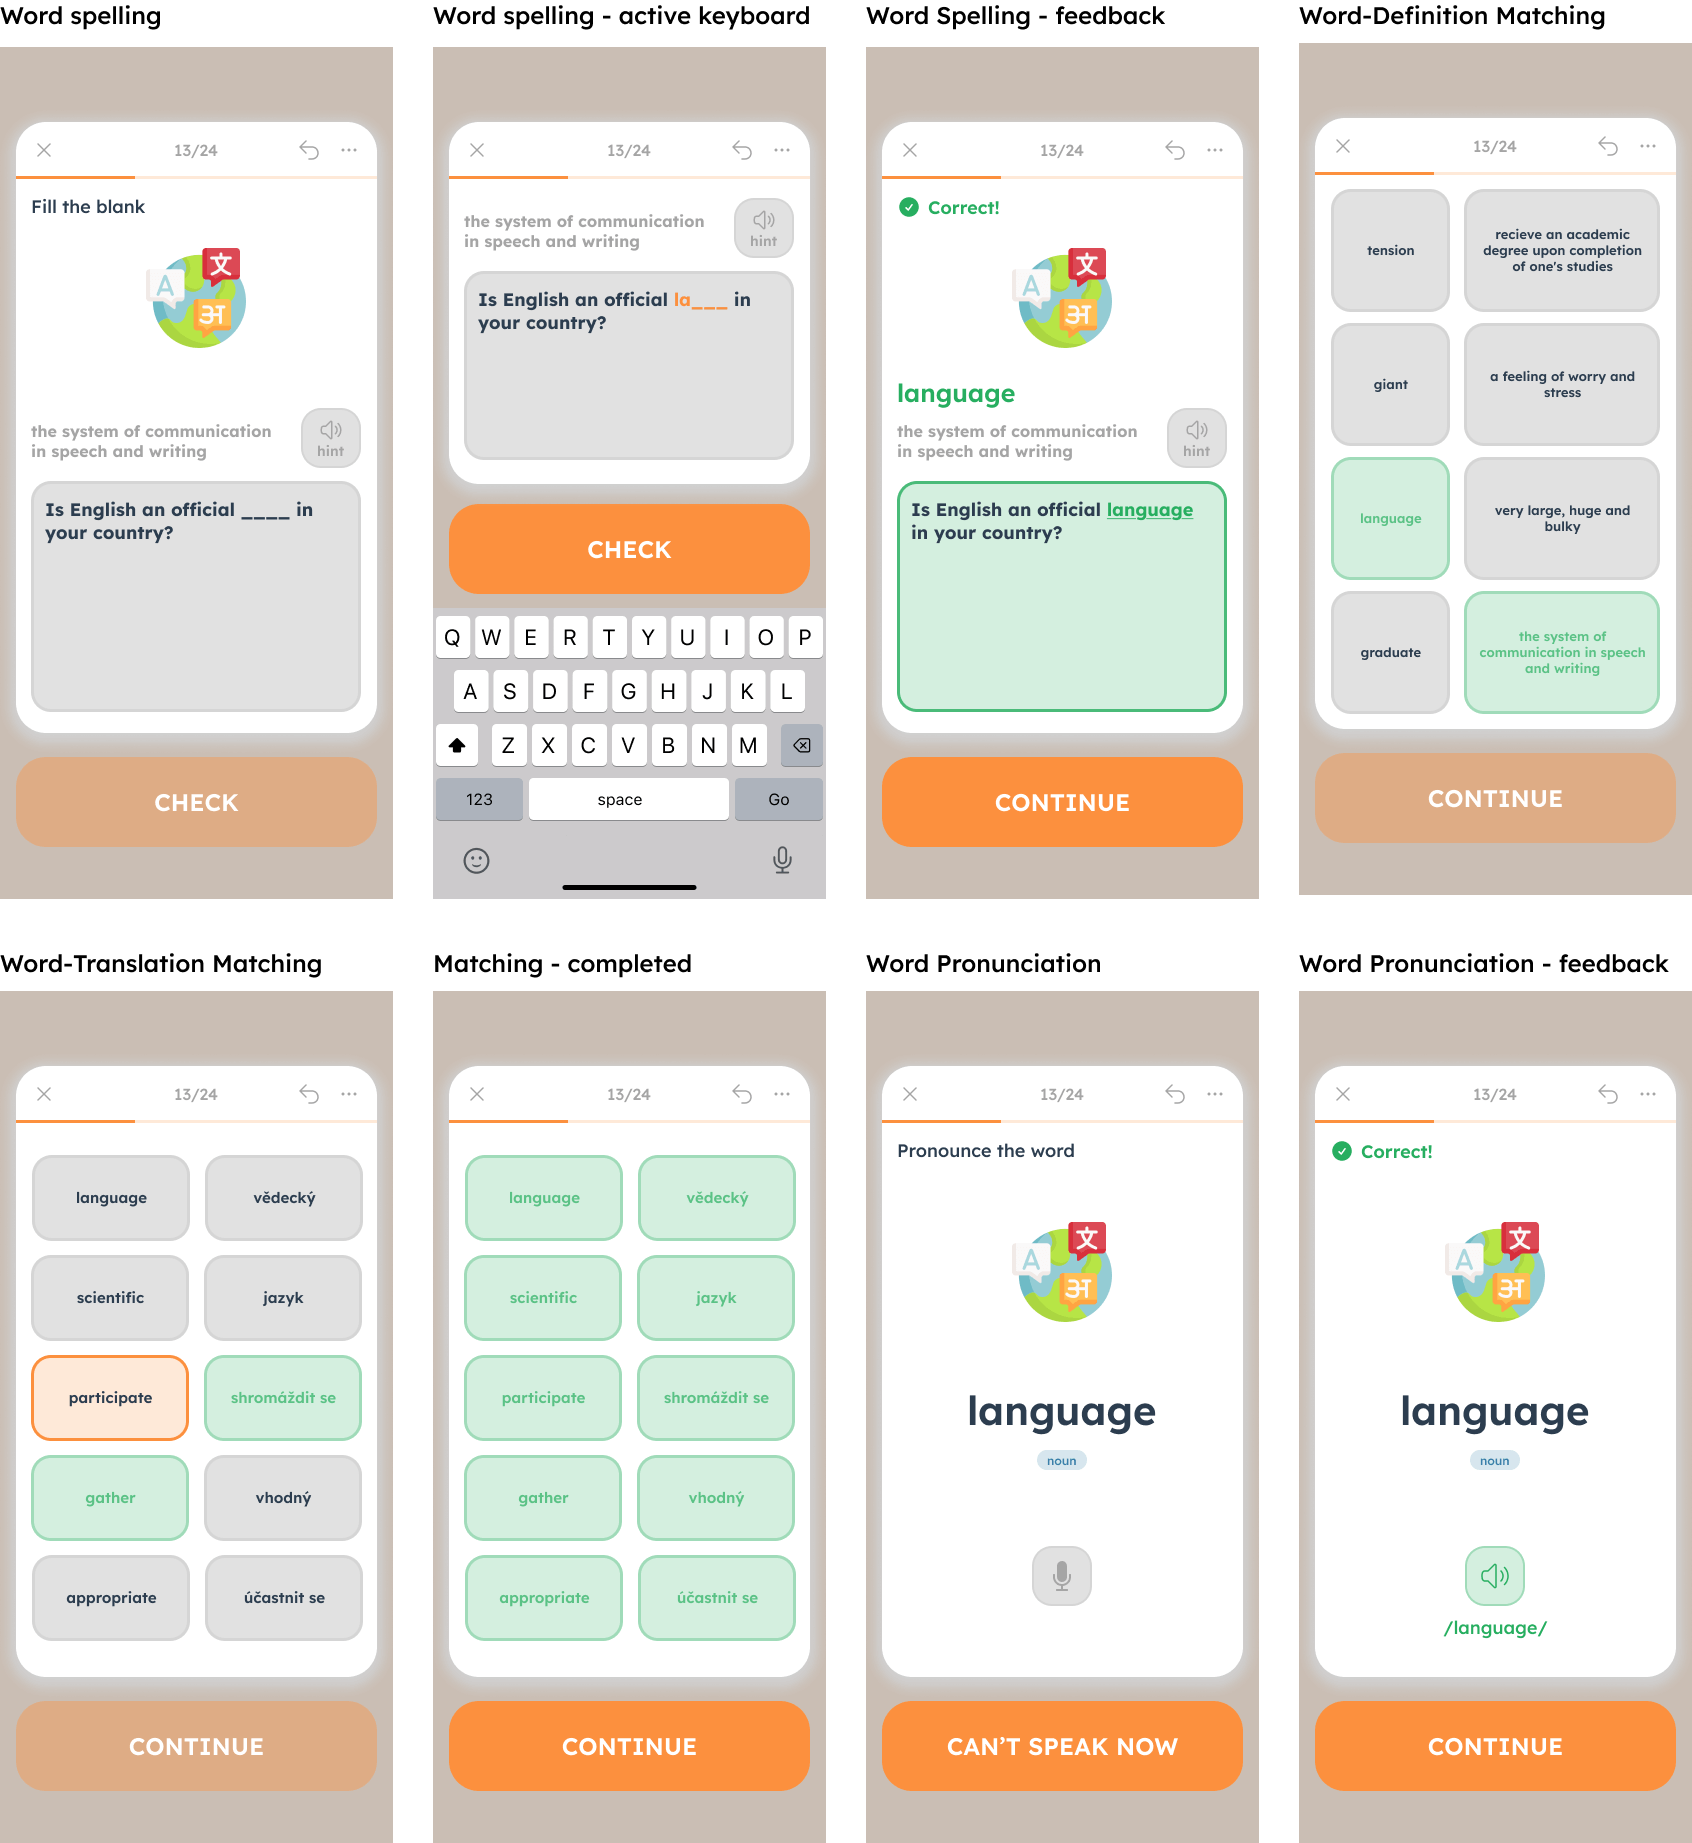
\includegraphics[width=1\textwidth]{src/figures/em-prototype-flashcards.png}
    \caption{English Mind - Prototype: Flashcard Types}
    \label{fig:em-prototype-flashcard-types}
\end{figure}

\subsubsection{Implementation Considerations}

The integration of new flashcard types requires careful consideration of both the spaced repetition system and the distribution of different card types during practice sessions.

To maintain the integrity of the existing spaced repetition system, only the basic meaning recognition flashcards will carry spaced repetition metadata and influence the scheduling of words. The additional flashcard types will serve as supplementary practice exercises without affecting the core SRS algorithm. This approach ensures the proven effectiveness of the current SRS remains unchanged, while additional practice types enhance learning without disrupting the established review schedule. Furthermore, this design allows user progress tracking to remain clear and consistent throughout the learning process.

The distribution of flashcard types within a practice session follows a structured approach that ensures varied practice while maintaining focus on core vocabulary acquisition through the primary flashcard type:

\begin{itemize}
    \item \textbf{Primary Flashcards:} Basic meaning recognition flashcards appear first in the daily queue, maintaining their role as the foundation of the spaced repetition learning system.
    
    \item \textbf{Supplementary Flashcards:} After completing the primary flashcards, users encounter the following types in randomized order:
    \begin{itemize}
        \item \textbf{Matching Flashcards:} Appear once for every five words in practice, grouping words into logical sets
        \item \textbf{Spelling Flashcards:} Randomly distributed throughout the supplementary practice
        \item \textbf{Pronunciation Flashcards:} Limited to newly introduced words and appear less frequently than other types
    \end{itemize}
\end{itemize}

\subsubsection{Expected Impact}

The diversification of flashcard types is expected to yield several benefits:

\begin{itemize}
    \item \textbf{Enhanced Engagement:} Variety in flashcard types reduces monotony and maintains user interest throughout longer practice sessions.
    
    \item \textbf{Comprehensive Learning and Retention:} Encountering words through diverse flashcard types (recognition, matching, spelling, and pronunciation) creates multiple memory pathways, leading to stronger and longer-lasting vocabulary mastery.
    
\end{itemize}

\subsection{Individual Word Progress Tracking}

Building upon the success of WordUp's individual word progress tracking (see Section \ref{sec:wordup-individual-word-progress-experience}), we propose implementing a visual progress indicator system that integrates seamlessly with English Mind's existing spaced repetition system. This feature provides users with clear, immediate feedback on their progress with each vocabulary item, helping them understand where they stand in the learning journey for specific words.

\subsubsection{Five-Stage Progress System}

The visual indicator system maps the existing spaced repetition intervals into five distinct stages. This system serves purely as a user-friendly representation of progress and does not modify the underlying SRS algorithm:


\begin{itemize}
    \item \textbf{Starting (Stage 1)}
    
    Represents words in their first 24 hours after introduction. These words are in the early stages of learning and require frequent review to establish basic recognition.
    
    \item \textbf{Familiarizing (Stage 2)}
    
    Covers words practiced between 1 day and 1 week. During this stage, words still require frequent reviews to build early recall strength and establish memory patterns.
    
    \item \textbf{Reinforcing (Stage 3)}
    
    Includes words with review intervals of 1-3 weeks. At this stage, users can recall words reliably, demonstrating consistent retention with moderate repetition intervals.
    
    \item \textbf{Strengthening (Stage 4)}
    
    Represents words practiced at 3-week to 3-month intervals. Users show strong confidence in recall, requiring significantly less frequent review as the word becomes well-established in long-term memory.
    
    \item \textbf{Almost Mastered (Stage 5)}
    
    Indicates words that have reached intervals of 3-8 months between reviews. These words are approaching full mastery, requiring only rare reviews to maintain retention. Once a word exceeds the 8-month interval, it will be marked as "known" and graduate from the regular review system.
\end{itemize}

\subsubsection{Visual Implementation}

The progress indicator appears in the top-left corner of primary flashcards (see Figure \ref{fig:em-prototype-word-progress}). It consists of five sequential boxes that fill progressively as the word advances through the stages, providing an intuitive visualization of progress. This design choice ensures the indicator is visible but not distracting from the primary learning task.

\begin{figure}[!h]
    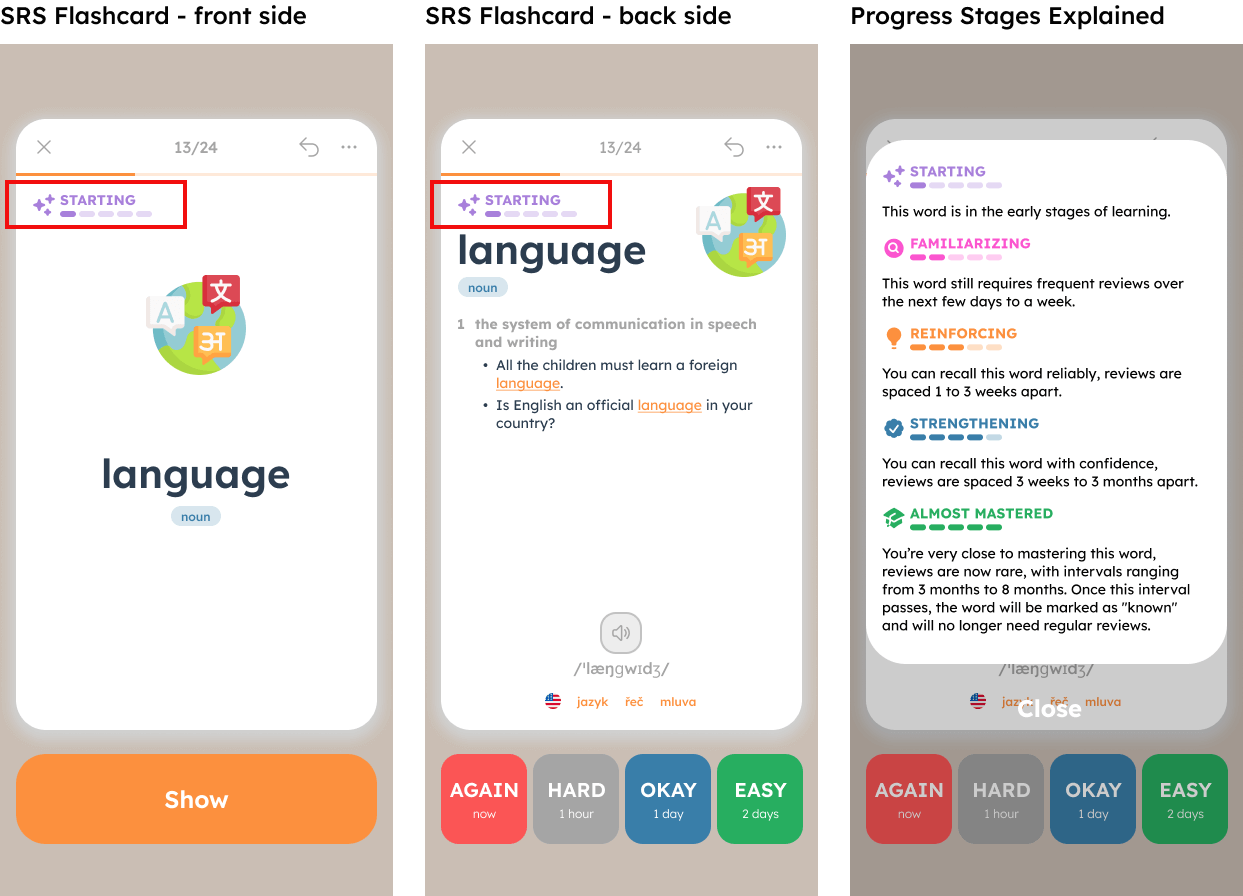
\includegraphics[width=1\textwidth]{src/figures/em-prototype-progress-system.png}
    \caption{English Mind - Prototype: Individual Word Progress Indicator (highlighted in red)}
    \label{fig:em-prototype-word-progress}
\end{figure}

\subsubsection{Integration with Existing SRS}

The progress tracking system is designed to work in harmony with the existing spaced repetition algorithm. Progress stages are determined automatically based on the word's current interval in the SRS system, with stages advancing or regressing according to review performance. This implementation leverages existing SRS metadata, requiring minimal additional computational overhead.

\subsubsection{Expected Impact}

The implementation of individual word progress tracking is expected to provide several benefits:

\begin{itemize}
    \item \textbf{Enhanced Motivation and Engagement:} Visual progress indicators create a game-like element that provides a sense of achievement as words advance through different stages.
    
    \item \textbf{Simplified Learning Metrics:} The staged system provides tangible feedback on the learning journey, making abstract concepts like spaced repetition more concrete and understandable.
\end{itemize}

\subsection{Post-Practice Review}

Drawing inspiration from Duolingo's successful implementation of post-practice feedback (see Section \ref{sec:duolingo-lesson-review}), we propose adding an engaging post-practice summary screen to English Mind. This feature provides immediate feedback and reinforcement after completing a practice session, helping users track their progress and maintain motivation.

\subsubsection{Post-Practice Review Screen Components}

The post-practice review screen consists of several key elements (see Figure \ref{fig:em-prototype-practice-review}):

\begin{itemize}
    \item \textbf{Practice Statistics}
    
    Clear visualization of practice session metrics including the number of words practiced and time spent practicing.
    
    \item \textbf{Mascot Interaction}
    
    The app's mascot appears with randomly selected poses to add personality to the user experience.
    
    \item \textbf{Motivational Messages}
    
    A rotating collection of encouraging messages that vary based on factors such as the number of words practiced, time spent practicing, and time of day.
    
    \item \textbf{Celebratory Animation}
    
    A confetti animation plays when the review screen appears, providing immediate positive reinforcement for completing the practice session. The animation is optimized to ensure smooth and lightweight performance across different devices.
\end{itemize}

\begin{figure}[!h]
    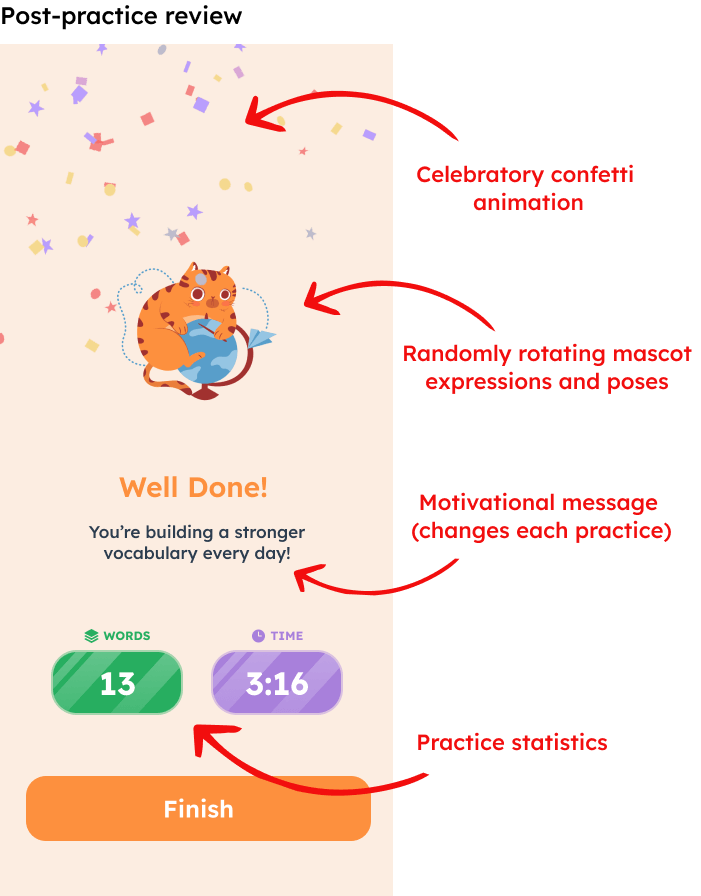
\includegraphics[width=0.8\textwidth]{src/figures/em-prototype-review.png}
    \caption{English Mind - Prototype: Post-Practice Review Screen}
    \label{fig:em-prototype-practice-review}
\end{figure}

\subsubsection{Expected Impact}

The implementation of a post-practice review screen is expected to:

\begin{itemize}
    \item \textbf{Increase Practice Completion:} The anticipation of positive feedback and celebration may motivate users to complete their practice sessions.
    
    \item \textbf{Boost User Satisfaction:} Immediate positive reinforcement through animations and encouraging messages creates a more rewarding experience.
\end{itemize}

\newpage

\section{Consistent Practice Motivation}
\label{sec:em-gamification-practice-motivation}
% This section focuses on features that encourage regular use

\subsection{Daily Goals and Streak System}
% Enhanced visualization of daily word goals
% Progress tracking throughout the day
% High-fidelity prototype for goal visualization
% Expected impact on daily engagement
% Daily streak tracking mechanism
% Streak protection features
% Notification strategy
% High-fidelity prototype for streak visualization
% Expected impact on long-term retention

\chapter{User Testing}

This chapter describes the methodology and results of user testing conducted on the previously proposed and designed gamification features for English Mind. The testing focused on evaluating the clarity, intuitiveness, and potential effectiveness of the new gamification elements.

\section{Testing Methodology}

Two distinct user groups were selected for testing to provide diverse perspectives. Group A consisted of participants with prior experience using language learning applications, while Group B included participants without significant experience in this area.

\begin{itemize}
    \item \textbf{Group A (Experienced Users):}
    \begin{itemize}
        \item 6 participants aged 18-45
        \item Regular users of apps like Duolingo, WordUp, or Duocards
        \item Familiar with gamification concepts through regular usage of language learning applications (even without knowing the formal terminology)
    \end{itemize}

    \item \textbf{Group B (Novice Users):}
    \begin{itemize}
        \item 6 participants aged 18-45
        \item Interest in learning English vocabulary
        \item Limited exposure to language learning applications
    \end{itemize}
\end{itemize}

The testing was conducted in a controlled, quiet environment where participants interacted with high-fidelity interactive prototypes on mobile devices. Each session lasted between 30-45 minutes and was documented through screen and audio recordings.

Data collection during the testing sessions combined several methods to gather comprehensive feedback about the gamification features. Participants were encouraged to think aloud while interacting with the prototype, sharing their thoughts and reactions to different elements. This verbal feedback was supplemented by observation notes documenting user behavior, particularly noting any points of confusion or excitement. After completing the test scenario (see Section \ref{sec:test-scenario}), participants filled out a structured questionnaire rating various aspects of the gamification features on a 5-point Likert scale (see Table \ref{tab:questionnaire}). The questionnaire focused on key metrics such as feature clarity, perceived usefulness, and likelihood of maintaining engagement.


\begin{table}[h]
    \centering
    \caption{User Testing Questionnaire}
    \label{tab:questionnaire}
    \makebox[\textwidth][c]{
        \begin{tabular}{|p{0.9\textwidth}|c|c|c|c|c|}
            \hline
            \multicolumn{6}{|l|}{\small 1 = Strongly Disagree, 2 = Disagree, 3 = Neutral, 4 = Agree, 5 = Strongly Agree} \\
            \hline
            \textbf{Question} & \textbf{1} & \textbf{2} & \textbf{3} & \textbf{4} & \textbf{5} \\
            \hline
            \multicolumn{6}{|l|}{\textbf{Practice Flashcards Experience}} \\
            \hline
            1. The different types of flashcards made practice more engaging & & & & & \\
            \hline
            2. Each flashcard type's instructions were clear and easy to understand & & & & & \\
            \hline
            3. The variety in flashcard types helped me learn vocabulary more effectively & & & & & \\
            \hline
            4. The distribution of different flashcard types felt well-balanced & & & & & \\
            \hline
            5. The five-stage individual word progress indicator was easy to understand & & & & & \\
            \hline
            6. Seeing my progress for individual words motivated me to practice more & & & & & \\
            \hline
            7. The individual word progress indicator's placement was visually clear without being distracting & & & & & \\
            \hline
            8. I found the progress tracking helpful for understanding my learning journey & & & & & \\
            \hline
            9. The practice statistics provided useful information about my session & & & & & \\
            \hline
            10. The celebratory animations made completing practice more rewarding & & & & & \\
            \hline
            11. The review screen motivated me to complete future practice sessions & & & & & \\
            \hline
            \multicolumn{6}{|l|}{\textbf{Streak System}} \\
            \hline
            12. The streak system's requirements were clear and easy to understand & & & & & \\
            \hline
            13. The visual states (active/at risk) effectively communicated streak status & & & & & \\
            \hline
            14. The celebration screen for maintaining streaks felt rewarding & & & & & \\
            \hline
            15. The requirement to learn one new word daily feels achievable & & & & & \\
            \hline
            16. The streak system would help me build a consistent practice habit & & & & & \\
            \hline
            17. I would be more likely to use the app regularly because of the streak feature & & & & & \\
            \hline
            \multicolumn{6}{|l|}{\textbf{Overall Experience}} \\
            \hline
            18. The gamification features enhanced my learning experience & & & & & \\
            \hline
            19. The features felt well-integrated with the app's educational purpose & & & & & \\
            \hline
            20. The gamification elements maintained my interest without being distracting & & & & & \\
            \hline
            21. I would recommend this app to others learning English vocabulary & & & & & \\
            \hline
            22. I would continue using this app for long-term vocabulary learning & & & & & \\
            \hline
        \end{tabular}
    }
\end{table}

\section{Test Scenario}
\label{sec:test-scenario}
The test scenario consists of two main phases: understanding the streak system and completing a practice session. This approach allows evaluation of both the gamification mechanics and their integration into the learning experience:

\begin{enumerate}
    \item \textbf{Phase 1: Streak System}
    \begin{itemize}
        \item Understanding streak activation and maintenance requirements
        \item Interpreting streak status indicators
        \item Initial feedback on motivational aspects
    \end{itemize}
    
    \item \textbf{Phase 2: Practice Flashcards Session}
    \begin{itemize}
        \item {Various Flashcard Types}
        \begin{itemize}
            \item Clarity of instructions for each flashcard type 
            \item Perceived value of variety in maintaining engagement
            \item Comfort level with each flashcard type's interaction method
        \end{itemize}

        \item {Individual Word Progress Tracking}
        \begin{itemize}
            \item Recognition and interpretation of the five-stage progress indicator
            \item Visibility and placement of the progress indicator
            \item Motivational impact of seeing word progress
        \end{itemize}

        \item {Post-Practice Review}
        \begin{itemize}
            \item Comprehension of practice statistics
            \item Impact of celebratory animations and mascot interactions
            \item Understanding of how the completed session affects their streak
        \end{itemize}
    \end{itemize}
\end{enumerate}

The testing process employs a think-aloud protocol, where participants verbalize their thoughts while interacting with the prototype. Initially, participants demonstrate their understanding of the streak system to the interviewer. They then proceed through a complete practice session, experiencing the integrated gamification elements. Throughout both phases, participants provide continuous feedback on interface clarity, emotional engagement, perceived long-term motivation potential, and any usability concerns. This structured approach enables comprehensive evaluation of both immediate user experience and potential sustained engagement with the application.

\newpage

\section{Results and Evaluation}

TODO...

\part{Implementation}
\chapter{Technology selection}
\chapter{Technology selection}
\chapter{User testing}
% --------------------------------------------

\appendix
\printindex
\bibliographystyle{unsrt}
\bibliography{src/references/bibliography}

\end{document}
